%preamble - package unclusion and set up
\documentclass[12pt,twoside,a4paper]{report}
\usepackage{etex}
% Select encoding of your inputs.
\usepackage[utf8]{inputenc}

% Make latex understand and use the typographic
% rules of the language used in the document.
\usepackage[english]{babel}

% Use the vector font Latin Modern which is going
% to be the default font in latex in the future.
\usepackage{lmodern}

% Choose the font encoding
\usepackage[T1]{fontenc}

% Use colour in tables
\usepackage[table]{xcolor}
\usepackage{array}
\usepackage{multirow}

% load a colour package
\usepackage{xcolor}
\definecolor{aaublue}{RGB}{33,26,82}% dark blue

% The standard graphics inclusion package
\definecolor{white}{RGB}{255,255,255} % define color white
\usepackage{graphicx}
\usepackage{adjustbox}

% Set up how figure and table captions are displayed
\usepackage{caption}
\captionsetup{
  font=footnotesize,% set font size to footnotesize
  labelfont=bf % bold label (e.g., Figure 3.2) font
}

% Enable row combination in tables
\usepackage{multirow}

% Make space between table lines and text
\renewcommand{\arraystretch}{1.5}

% Enable commands like \st (strike out) and \hl (high light)
\usepackage{soul}

% Make the standard latex tables look so much better
\usepackage{array,booktabs}

% Enable the use of frames around, e.g., theorems
% The framed package is used in the example environment
\usepackage{framed}
\usepackage{colortbl}
\usepackage{longtable}
\usepackage{xcolor}
\usepackage{textcomp}

%%%%%%%%%%%%%%%%%%%%%%%%%%%%%%%%%%%%%%%%%%%%%%%%
% Mathematics
%%%%%%%%%%%%%%%%%%%%%%%%%%%%%%%%%%%%%%%%%%%%%%%%
% Defines new environments such as equation,
% align and split 
\usepackage{amsmath}
\usepackage{relsize}
% Adds new math symbols
\usepackage{amssymb}
% Use theorems in your document
% The ntheorem package is also used for the example environment
% When using thmmarks, amsmath must be an option as well. Otherwise \eqref doesn't work anymore.
\usepackage[framed,amsmath,thmmarks]{ntheorem}

%%%%%%%%%%%%%%%%%%%%%%%%%%%%%%%%%%%%%%%%%%%%%%%%
% Page Layout
%%%%%%%%%%%%%%%%%%%%%%%%%%%%%%%%%%%%%%%%%%%%%%%%
% Change margins, papersize, etc of the document
\usepackage[
  left=25mm,% left margin on an odd page %tidligere 25mm for baade right og left
  right=25mm,% right margin on an odd page
  top=35mm,
  ]{geometry}
  
% Modify how \chapter, \section, etc. look
% The titlesec package is very configureable
\usepackage{titlesec}
\makeatletter
\def\ttl@mkchap@i#1#2#3#4#5#6#7{%
    \ttl@assign\@tempskipa#3\relax\beforetitleunit
    \vspace{\@tempskipa}%<<<<<< REMOVE THE * AFTER \vspace
    \global\@afterindenttrue
    \ifcase#5 \global\@afterindentfalse\fi
    \ttl@assign\@tempskipb#4\relax\aftertitleunit
    \ttl@topmode{\@tempskipb}{%
        \ttl@select{#6}{#1}{#2}{#7}}%
    \ttl@finmarks  % Outside the box!
    \@ifundefined{ttlp@#6}{}{\ttlp@write{#6}}}
\makeatother

\titlespacing{\chapter}{0pt}{0pt}{10pt}
\titlespacing{\section}{0pt}{0pt}{-5pt}
\titlespacing{\subsection}{0pt}{8pt}{-5pt}
\titlespacing{\subsubsection}{0pt}{6pt}{-10pt}

\titleformat*{\section}{\normalfont\Large\bfseries\color{aaublue}}
\titleformat*{\subsection}{\normalfont\large\bfseries\color{aaublue}}
\titleformat*{\subsubsection}{\normalfont\normalsize\bfseries\color{aaublue}}

\usepackage{titlesec, blindtext, color}
%\color{gray75}{gray}{0.75}
\newcommand{\hsp}{\hspace{20pt}}
\titleformat{\chapter}[hang]{\Huge\bfseries}{\thechapter\hsp\textcolor{aaublue}{|}\hsp}{0pt}{\Huge\bfseries}

% Change the headers and footers
\usepackage{fancyhdr}
\setlength{\headheight}{15pt}
\pagestyle{fancy}
\fancyhf{} %delete everything
\renewcommand{\headrulewidth}{0pt} %remove the horizontal line in the header
\fancyhead[RO,LE]{\color{aaublue}\small\nouppercase\leftmark} %even page - chapter title
\fancyhead[LO]{}
\fancyhead[RE]{} 
\fancyhead[CE]{}
\fancyhead[CO]{}
\fancyfoot[RE,LO]{\thepage}
\fancyfoot[LE,RO]{Gr. 834} %page number on all pages
\fancyfoot[CE,CO]{}

% change first page of all chapters header and footer to fancy style
\makeatletter
\let\ps@plain\ps@fancy
\makeatother

% Do not stretch the content of a page. Instead,
% insert white space at the bottom of the page
\raggedbottom

% Enable arithmetics with length. Useful when typesetting the layout.
\usepackage{calc}

%%%%%%%%%%%%%%%%%%%%%%%%%%%%%%%%%%%%%%%%%%%%%%%%
% Bibliography
%%%%%%%%%%%%%%%%%%%%%%%%%%%%%%%%%%%%%%%%%%%%%%%%
%setting references (using numbers) and supporting i.a. Chicargo-style:
%\usepackage[citestyle=authoryear,natbib=true]{biblatex}
\usepackage[backend=biber]{biblatex}
%\usepackage{etex}
%\usepackage{etoolbox}
%\usepackage{keyval}
%\usepackage{ifthen}
%\usepackage{url}
%\usepackage{csquotes}
%\usepackage[backend=biber, url=true, doi=true, style=numeric, sorting=none]{biblatex}
%\addbibresource{setup/bibliography.bib}
\bibliography{setup/bibliography.bib}

\usepackage[utf8]{inputenc}
\usepackage[english]{babel}

\usepackage{comment}

%\usepackage[
%backend=biber,
%style=numeric,
%sorting=ynt
%]{biblatex}
%\addbibresource{setup/bibliography.bib}

%%%%%%%%%%%%%%%%%%%%%%%%%%%%%%%%%%%%%%%%%%%%%%%%
% Misc
%%%%%%%%%%%%%%%%%%%%%%%%%%%%%%%%%%%%%%%%%%%%%%%%

%%% Enables the use FiXme refferences. Syntax: \fxnote{...} %%%
\usepackage[footnote, draft, english, silent, nomargin]{fixme}
%With "final" instead of "draft" an error will ocure for every FiXme under compilation.

%%% allows use of lorem ipsum (generate i.e. pagagraph 1 to 5 with \lipsum[1-5]) %%%
\usepackage{lipsum}

%%% Enables figures with text wrapped tightly around it %%%
\usepackage{wrapfig}

%%% Section debth included in table of contents (1 = down to sections) %%%
\setcounter{tocdepth}{1}

%%% Section debth for numbers (1 = down to sections) %%%
\setcounter{secnumdepth}{1}

\usepackage{tocloft}
\setlength{\cftbeforetoctitleskip}{0 cm}
\renewcommand{\cftpartpresnum}{Part~}
\let\cftoldpartfont\cftpartfont
\renewcommand{\cftpartfont}{\cftoldpartfont\cftpartpresnum}

%%%%%%%%%%%%%%%%%%%%%%%%%%%%%%%%%%%%%%%%%%%%%%%%
% Hyperlinks
%%%%%%%%%%%%%%%%%%%%%%%%%%%%%%%%%%%%%%%%%%%%%%%%

% Enable hyperlinks and insert info into the pdf
% file. Hypperref should be loaded as one of the 
% last packages
\usepackage{nameref}
\usepackage{hyperref}
\hypersetup{%
	%pdfpagelabels=true,%
	plainpages=false,
	pdfauthor={Author(s)},%
	pdftitle={Title},%
	pdfsubject={Subject},%
	bookmarksnumbered=true,%
	colorlinks,%
	citecolor=aaublue,%
	filecolor=aaublue,%
	linkcolor=aaublue,% you should probably change this to black before printing
	urlcolor=aaublue,%
	pdfstartview=FitH%
}

% remove all indentations
\setlength\parindent{0pt}
\parskip 5mm
\usepackage{verbatim}

\definecolor{Gra}{RGB}{230,230,230}

%creates a nice-looking C#-text
\newcommand{\CC}{C\nolinebreak\hspace{-.05em}\raisebox{.3ex}{\scriptsize\text \#} }

%enables multi column lists
\usepackage{multicol}

%enables code-examples
\usepackage{listings}

\definecolor{coolblue}{RGB}{32,95,128}
\definecolor{mygreen}{rgb}{0,0.6,0}
\definecolor{mygray}{rgb}{0.5,0.5,0.5}
\definecolor{mymauve}{rgb}{0.58,0,0.82}
\usepackage{textcomp}
\definecolor{listinggray}{gray}{0.9}
\definecolor{lbcolor}{rgb}{0.9,0.9,0.9}

\lstset{
backgroundcolor=\color{lbcolor},
	tabsize=4,
	rulecolor=,
	language=C,
        basicstyle=\scriptsize,
        upquote=true,
        aboveskip={1.5\baselineskip},
        columns=fixed,
        showstringspaces=false,
        extendedchars=true,
        breaklines=true,
        prebreak = \raisebox{0ex}[0ex][0ex]{\ensuremath{\hookleftarrow}},
        frame=single,
        showtabs=false,
        numbers=left,
        captionpos=b,
        numbersep=5pt,
        numberstyle=\tiny\color{mygray},
        showspaces=false,
        showstringspaces=false,
        identifierstyle=\ttfamily,
        keywordstyle=\color[rgb]{0,0,1},
        commentstyle=\color[rgb]{0.133,0.545,0.133},
        stringstyle=\color[rgb]{0.627,0.126,0.941},
}

%% ADD MATLAB COLOR CODE
\lstdefinestyle{custommatlab}{
	backgroundcolor=\color{lbcolor},
	tabsize=4,
	rulecolor=,
	language=Matlab,
	basicstyle=\scriptsize,
	upquote=true,
	aboveskip={1.5\baselineskip},
	columns=fixed,
	showstringspaces=false,
	extendedchars=true,
	breaklines=true,
	prebreak = \raisebox{0ex}[0ex][0ex]{\ensuremath{\hookleftarrow}},
	frame=single,
	showtabs=false,
	numbers=left,
	captionpos=b,
	numbersep=5pt,
	numberstyle=\tiny\color{mygray},
	showspaces=false,
	showstringspaces=false,
	identifierstyle=\ttfamily,
	keywordstyle=\color[rgb]{0,0,1},
	commentstyle=\color[rgb]{0.133,0.545,0.133},
	stringstyle=\color[rgb]{0.627,0.126,0.941},   
}
\lstdefinestyle{custommatlabinline}{
	style=custommatlab,
	basicstyle=\small,
}

\usepackage{float}
\usepackage{caption}
\usepackage{subcaption}
\usepackage{siunitx}
\sisetup{decimalsymbol=comma}
\sisetup{detect-weight}

\usepackage{enumitem}

% Figures - TIKZ
\usepackage{tikz}
\usetikzlibrary{shapes,arrows}
\usepackage[americanresistors,americaninductors,americancurrents, americanvoltages]{circuitikz}

% Wall of text logo
\newcommand{\walloftextalert}[0]{\includegraphics[width=\textwidth]{walloftext.png}}

\usepackage{pdfpages}
\usepackage{lastpage}
\usepackage{epstopdf}

\setlength{\headheight}{21pt}

\hfuzz=\maxdimen
\tolerance = 10000
\hbadness  = 10000

\usepackage{siunitx}
\graphicspath{{./figures/}}

\usepackage{todonotes}

\usepackage{nomencl}
\makenomenclature


\usepackage[toc,xindy]{glossaries}
\makeglossaries


\usepackage{ifthen}
\renewcommand{\nomgroup}[1]{%
	\ifthenelse{\equal{#1}{T}}{\item[\textbf{\Large Terminology}]}{%
	\ifthenelse{\equal{#1}{A}}{\item[\textbf{\Large Acronyms}]}{%
	\ifthenelse{\equal{#1}{R}}{\item[\textbf{\Large Reference Frames}]}{%
	\ifthenelse{\equal{#1}{S}}{\item[\textbf{\Large Symbols}]}{}}
}}}

\setlength{\nomlabelwidth}{4.5cm} % set spacing between symbol and description

\renewcommand{\nompreamble}{
	\section*{Notations}

Vectors used have a bold typeface.  
\begin{equation*}
\textbf{v}
\end{equation*}
Matrices are underlined.
\begin{equation*}
\underline{A}
\end{equation*}

Cross product operations can be evaluated by taking the skew symmetric matrix of the left vector and executing a matrix multiplication. The skew symmetric matrix of $\textbf{v}$ is denoted as $\underline{v}^\times$
\begin{equation*}
	\textbf{w} = \textbf{u} \times \textbf{v} = \underline{u}^\times \textbf{v}
\end{equation*}
Matrix transposition is denoted as
\begin{equation*}
\underline{A}^T
\end{equation*}
If a non-square matrix has to undergo an operation similar to inversion, Moore-Penrose pseudoinverse is used. Pseudoinverse matrix is indicated as $\underline{A}^\dagger$. If the matrix satisfies $rank(\underline{A}) = min(m,n)$ and $m < n$, the left pseudoinverse is used as follows
\begin{equation*}
\underline{A}^\dagger    =   (\underline{A}^T \underline{A} )^{-1} \underline{A}^T 
\end{equation*}

If $n < m$, the right pseudoinverse is used as follows

\begin{equation*}
 \underline{A}^\dagger    =  \underline{A}^T  (\underline{A} \underline{A}^T)^{-1}
\end{equation*}


The majority of equations are expressed in body-fixed frame (BFF). Unless it's not explicitly noted, the matrices and vectors are expressed in BFF. In case the expression is in earth centered inertial frame (ECI), it is noted in the superscript as 

\begin{equation*}
\vec{XY}^{[I]}
\end{equation*}

The rotation quaternion between frames use the subscript to denote the frame where the transformation is done from, the superscript is the symbol of the frame being transformed into. In case the frame symbols are not present, it should be interpreted as a transformation from inertial frame to body frame.

\begin{equation*}
\vec{^s_i q(t)}
\end{equation*}

Rotation matrix corresponding to rotation matrix $\vec{^s_i q(t)}$ is denoted as
\begin{equation*}
\underline{R}(\vec{^s_i q(t)})
\end{equation*}}

%macros - please read this file
%%%%%%%%%%%%%%%%%%%%%%%%%%%%%%%%%%%%%%%%%%%%%%%%%%%%%
%             UNITS, EQUATIONS AND TEXT             %
%%%%%%%%%%%%%%%%%%%%%%%%%%%%%%%%%%%%%%%%%%%%%%%%%%%%%
%Units:
\newcommand{\unit}[1]{&& \left[\si{#1}\right]} %\newcommand{\unit}[1]{[\si{#1}]}             <<| Use these if you want equations to be
\newcommand{\unitWh}[1]{[\si{#1}]}             %\newcommand{\eq}[2]{&&\si{#1} &= \si{#2}&&}  <<| centered.. .. will appear scrambled
\newcommand{\numUnit}[1]{\ \si{#1}&}           %                                               | from one equation to the next though..
%Equation:                                     %                                               | and does not work with long equations.. :/
\newcommand{\eq}[2]{\si{#1} &= \si{#2}}
\newcommand{\arw}{&& &\Updownarrow&&}
\newcommand{\eqOne}[2]{\si{#1} &= \si{#2} &\nonumber\\}
\newcommand{\eqTwo}[1]{&\ \ \ \ \si{#1}&}
%Text:
\newcommand{\tx}[1]{\text{#1}}
%Vectors
\renewcommand{\vec}[1]{\boldsymbol{\mathbf{#1}}}
%Vertical line in equations ie. |_x=y (whereTwo stacks two equalities at the line)
\newcommand{\where}[1]{ \left.\rule{0cm}{.5cm}\right\vert\rule{0cm}{.4cm}_{\substack{\rule{0cm}{.15cm}\\ \si{#1} }} }
\newcommand{\whereTwo}[2]{ \left.\rule{0cm}{.67cm}\right\vert\rule{0cm}{.5cm}_{\substack{\si{#1} \rule{0cm}{.19cm}\\\vspace{-.1cm}\\ \si{#2}}} }

%%%%%%%%%%%%%%%%%%%%%%%%%%%%%%%%%%%%%%%%%%%%%%%%%%%%%
%                 TIKZ SETTINGS                     %
%%%%%%%%%%%%%%%%%%%%%%%%%%%%%%%%%%%%%%%%%%%%%%%%%%%%%
\tikzset{
  block/.style    = {draw, thick, rectangle,
                     minimum height = 3em,
                     minimum width = 3em},
  sum/.style      = {draw, circle}, % Adder
}

%%%%%%%%%%%%%%%%%%%%%%%%%%%%%%%%%%%%%%%%%%%%%%%%%%%%%
%                  REFERENCES                       %
%%%%%%%%%%%%%%%%%%%%%%%%%%%%%%%%%%%%%%%%%%%%%%%%%%%%%

%Chapter
\newcommand{\Chapref}[1]{\emph{Chapter \ref{#1}}}
\newcommand{\chapref}[1]{\emph{chapter \ref{#1}}}
%Section
\newcommand{\Secref}[1]{\emph{Section \ref{#1}}}
\newcommand{\secref}[1]{\emph{section \ref{#1}}}
%subSection
\newcommand{\Subsecref}[1]{\emph{Subsection \ref{#1}}}
\newcommand{\subsecref}[1]{\emph{subsection \ref{#1}}}
%Appendix
\newcommand{\Appref}[1]{\emph{Appendix \ref{#1}}}
\newcommand{\appref}[1]{\emph{appendix \ref{#1}}}
%Listings
\newcommand{\Coderef}[1]{\emph{Listings: \ref{#1}}}
\newcommand{\coderef}[1]{\emph{listings: \ref{#1}}}
%Figure:
\newcommand{\Figref}[1]{\emph{Figure \ref{#1}}}
\newcommand{\figref}[1]{\emph{figure \ref{#1}}}
%Table:
\newcommand{\Tableref}[1]{\emph{Table \ref{#1}}}
\newcommand{\tableref}[1]{\emph{table \ref{#1}}}

%Expressions:
\newcommand{\Expr}[1]{\emph{Expression (\ref{#1})}}
\newcommand{\expr}[1]{\emph{expression (\ref{#1})}}

%Equations:
%1 equation:
\newcommand{\Eqref}[1]{\emph{Equation (\ref{#1})}}
\renewcommand{\eqref}[1]{\emph{equation (\ref{#1})}}
%2 equations:
\newcommand{\EqrefTwo}[2]{\emph{Equation (\ref{#1})} and \emph{(\ref{#2})}}
\newcommand{\eqrefTwo}[2]{\emph{equation (\ref{#1})} and \emph{(\ref{#2})}}
%3 equations:
\newcommand{\EqrefThree}[3]{\emph{Equation (\ref{#1})}, \emph{(\ref{#2})} and \emph{(\ref{#3})}}
\newcommand{\eqrefThree}[3]{\emph{equation (\ref{#1})}, \emph{(\ref{#2})} and \emph{(\ref{#3})}}
%4 equations:
\newcommand{\EqrefFour}[4]{\emph{Equation (\ref{#1})}, \emph{(\ref{#2})}, \emph{(\ref{#3})} and \emph{(\ref{#4})}}
\newcommand{\eqrefFour}[4]{\emph{equation (\ref{#1})}, \emph{(\ref{#2})}, \emph{(\ref{#3})} and \emph{(\ref{#4})}}
%5 equations:
\newcommand{\EqrefFive}[5]{\emph{Equation (\ref{#1})}, \emph{(\ref{#2})}, \emph{(\ref{#3})}, \emph{(\ref{#4})} and \emph{(\ref{#5})}}
\newcommand{\eqrefFive}[5]{\emph{equation (\ref{#1})}, \emph{(\ref{#2})}, \emph{(\ref{#3})}, \emph{(\ref{#4})} and \emph{(\ref{#5})}}
%6 equations:
\newcommand{\EqrefSix}[6]{\emph{Equation (\ref{#1})}, \emph{(\ref{#2})}, \emph{(\ref{#3})}, \emph{(\ref{#4})}, \emph{(\ref{#5})} and \emph{(\ref{#6})}}
\newcommand{\eqrefSix}[6]{\emph{equation (\ref{#1})}, \emph{(\ref{#2})}, \emph{(\ref{#3})}, \emph{(\ref{#4})}, \emph{(\ref{#5})} and \emph{(\ref{#6})}}
%7 equations:
\newcommand{\EqrefSeven}[7]{\emph{Equation (\ref{#1})}, \emph{(\ref{#2})}, \emph{(\ref{#3})}, \emph{(\ref{#4})}, \emph{(\ref{#5})}, \emph{(\ref{#6})} and \emph{(\ref{#7})}}
\newcommand{\eqrefSeven}[7]{\emph{equation (\ref{#1})}, \emph{(\ref{#2})}, \emph{(\ref{#3})}, \emph{(\ref{#4})}, \emph{(\ref{#5})}, \emph{(\ref{#6})} and \emph{(\ref{#7})}} % :TIP: If you are using TeXstudio you can open
                         %     the file by Ctrl+LeftClick on setup/macros.tex
\begin{document}         %     If the file doesn't exist, you will be asked
	
\pagestyle{empty} %disable headers and footers
\pagenumbering{roman} %use roman page numbering in the frontmatter I II...
\fancyfoot[RE,LO]{17gr834} %page number on all pages
\fancyfoot[LE,RO]{\thepage}
\fancyhead[LE,LO,RE,RO]{}

\pdfbookmark[0]{Front Page}{label:forside}%
\begin{titlepage}
  \addtolength{\hoffset}{0.5\evensidemargin-0.5\oddsidemargin} %set equal margins on the frontpage - remove this line if you want default margins
  \noindent%
  \begin{tabular}{@{}p{\textwidth}@{}}
    \toprule[2pt]
    \midrule
    \vspace{0.2cm}
    \begin{center}
    \Huge{\textbf{
      % CubeSat Formation Flying
      Fault Tolerant Attitude Control of a Pico-Satellite Equipped with Reaction Wheels
      and Magnetorquers% insert your title here
    }}
    \end{center}
%    \begin{center}
%      \Large{
%
%      }
%    \end{center}
    \vspace{0.2cm}\\
    \midrule
    \toprule[2pt]
  \end{tabular}
   \vspace{0.55 cm}
  \begin{figure}[!ht]
\centering
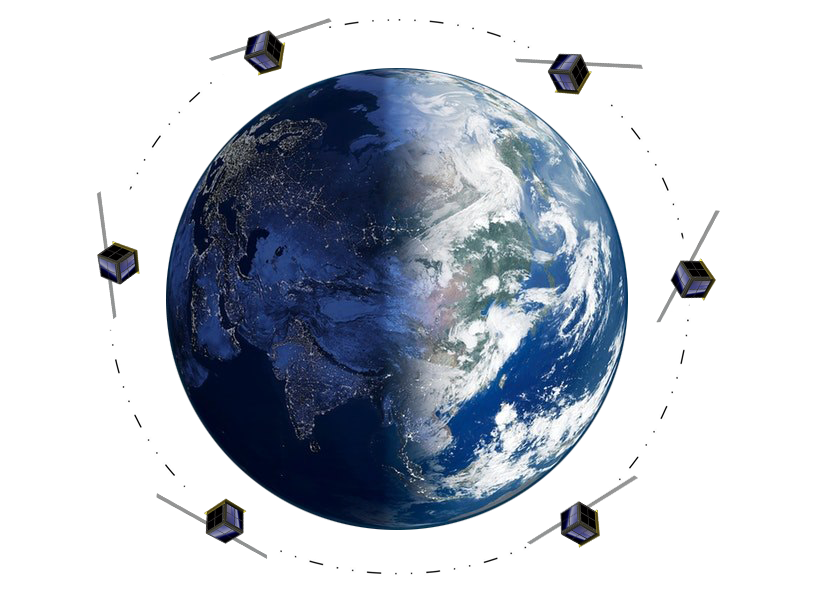
\includegraphics[width=0.8\textwidth]{figures/c1}
\label{fig:forside}
\end{figure}
  \vspace{0.6 cm}
  \begin{center}
%    {\large
%      2. Semester Project Report %Insert document type (e.g., Project Report)
%    }\\
    \vspace{0.2cm}
    {\Large
      Group 18gr1033 %Insert your group name or real names here
    }
  \end{center}
  \begin{center}
  Aalborg University\\
  Control \& Automation\\
  Fredrik Bajers Vej 7\\
  DK-9220 Aalborg
  \end{center}
\end{titlepage}

\clearpage	%frontpage doh
\cleardoublepage
%\begin{document} 
%\thispagestyle{empty}
%\begin{titlepage}
\begin{nopagebreak}
{\samepage 

\begin{tabular}{r}
\parbox{\textwidth}{  \raisebox{-15mm}{
\includegraphics[height=3cm]{figures/aaulogo-en.png}}
\hfill \hspace{2cm} \parbox{8cm}{\begin{tabular}{l} %4.90
{\small \textbf{\textcolor{aaublue}{\colorbox{white}{10\textsuperscript{th} Semester, Project}}}}\\
{\small \textbf{\textcolor{aaublue}{Technical Faculty of IT and Design}}}\\
{\small \textbf{\textcolor{aaublue}{Department of
	Electronics Systems}}}\\ 
{\small \textbf{\textcolor{aaublue}{Control and Automation}}}\\
{\small \textcolor{aaublue}{Fredrik Bajers Vej 7C}} \\
{\small \textcolor{aaublue}{9220 Aalborg}} \\
{\small \textcolor{aaublue}{\emph{en.aau.dk/education/master/control-automation}}}
\end{tabular}}}
\end{tabular}

\begin{tabular}{cc}
\parbox{7cm}{

\textbf{Title:}

Fault Tolerant Attitude Control of a Pico-Satellite Equipped with Reaction Wheels
and Magnetorquers \\ %\fxnote{Input project title}\\

\textbf{Theme:}

\small{
 Master thesis\\
}


\parbox{8cm}{


\textbf{Project Period:}\\
P10, Spring 2018\\
01/02/2018 - 07/06/2018\\
   
\textbf{Project Group:}\\
18gr1033\\ %\fxnote{Input group number}
  
\textbf{Participants:}\\
- Dániel Bolgár  \\
- Nikolaos Biniakos\\
- Alexandru-Cosmin Nicolae\\

\textbf{Supervisors:}\\
Jesper Abilgaard Larsen \\ %\fxnote{Input supervisor}
}\\


\textbf{Pages:} \\
\textbf{Appendices:} 2 (4 pages)\\
\textbf{Attached:} 1 zip file\\
\textbf{Concluded:} 07/06/2018\\

\vfill } &
\parbox{7cm}{
  \vspace{.15cm}
  \hfill
  \begin{tabular}{l}
  {\textbf{Synopsis}}\bigskip \\
  \fbox{
    \parbox{6.5cm}{\bigskip
     {\vfill{\small This report describes the design and simulation of a control system on a AAU-CubeSat, which is a pico- satellite used for Low Earth Orbit flight.

The objective is to use a flight formation for monitoring Greenland, by having eight satellites equally distributed in orbit.

Two controllers must be designed, one to control the angle between the satellites using the drag force, and one for attitude control.  The drag force applied on the satellite depends on the cross section area which can be controlled using the orientation of the satellite.

A linear and a non-linear control method have been designed in order to compare the differences between them.  
     \bigskip}}
     }}
   \end{tabular}}
\end{tabular}} %\vspace{1cm}



\end{nopagebreak}
%\end{titlepage}
%\end{document}
\cleardoublepage
\chapter*{Preface}
This report has been written by group 1033 during fourth semester in Control and Automation MSc in Aalborg University, Department of Electronic Systems during the period from February 2018 to June 2018. It is written as a Master's thesis for the Control and Automation Master's program. 

A nomenclature is included presenting the acronyms, symbols and terminology used throughout the thesis.  Quotes are inside quotation marks and are cursive.

The authors would like to thank Associate Professor Jesper Abilgaard Larsen for supervising. The authors furthermore would like to thank the students involved in the development of the AAUSAT Simulink Library.

% References made before a full stop regards the sentence and reference after full stop regards the paragraph.
Attached to report is a zip file with:
\begin{itemize}
	\item The MATLAB code 
	\item Simulink models
\end{itemize}
\vspace{2cm}

\textbf{Report by:}\\
\vspace{-5pt}
\begin{table}[H]
	\centering
	\begin{tabular}{c c c}
		\underline{\phantom{JAERJAERJAERJAERGO}} & \phantom{cookies} & \underline{\phantom{JAERJAERJAERJAERGO}} \\
		 	Dániel Bolgár	& \phantom{cookies} &  Nikolaos Biniakos	\\
		&&\\
		\multicolumn{3}{c}{\underline{\phantom{JAERJAERJAERJAERGO}}}\\
		\multicolumn{3}{c}{Alexandru-Cosmin Nicolae}\\				
						
	\end{tabular}
\end{table}


\pagebreak


\tableofcontents         %     weath2 er or not you want to create it.
\cleardoublepage

\pagenumbering{arabic} %use arabic page numbering in the mainmatter
\fancyfoot[RO,LE]{\thepage \text{ of} \pageref{LastPage}}
\fancyfoot[RE,LO]{17gr834}
\fancyhead[RE,LO]{}
\fancyhead[RE,LO]{\color{aaublue}\small\nouppercase\leftmark} %even page - chapter title
\pagestyle{fancy}

%||||||||||||||||||||||||||||||||||||||||||||||||||||||||||||||||
%|||||||       Set Section and chapters as input below   ||||||||
%||||||||||||||||||||||||||||||||||||||||||||||||||||||||||||||||

\listoftodos
\printglossary
\printnomenclature \todo{make nomenclature and glossary to work}
\chapter{Introduction}\label{chap:Introduction}

Satellites are no longer the privilege of just a handful of economic powerhouses such as nations or mega companies. While the satellites themselves can be engineered to be relatively cheap, there is no avoiding the high cost of putting the satellite into orbit. Many efforts were made recently to reduce this cost. The cost is highly dependent on the weight of the satellite, thus by minimizing the weight 

\section{Problem statement}

\newglossaryentry{AAUSAT}{name={AAUSAT},description={Cool-ass picosatellite}}

\section{Use-case}\label{sec:useCase}



\chapter{Satellite Modeling}
\todo{maybe some intro}
\section{Reference Frames}

\nomenclature[A]{\textbf{ECI}}{Earth Centered Inertial Frame}
\nomenclature[A]{\textbf{ECEF}}{Earth Centered Earth Fixed Frame}
\nomenclature[A]{\textbf{SBRF}}{Satellite Body Reference Frame}

Using different reference frame for different calculations can simplify equations. Values in one reference frame can be converted into the other by using the proper transformations.
Inertial frames of reference are frames where Newton's 3 laws of dynamics apply.
The most used reference frames for Earth-orbiting satellites are Earth Centered Inertial Frame (ECI), Earth Centered Earth Fixed Frame (ECEF), Orbit Frame, Satellite Body Reference Frame (SBRF)  \cite{ref1} \cite{ref2}. Figure \ref{fig:frames} provides a visualization of the frames.

\begin{figure}[h!]
	\centering 
	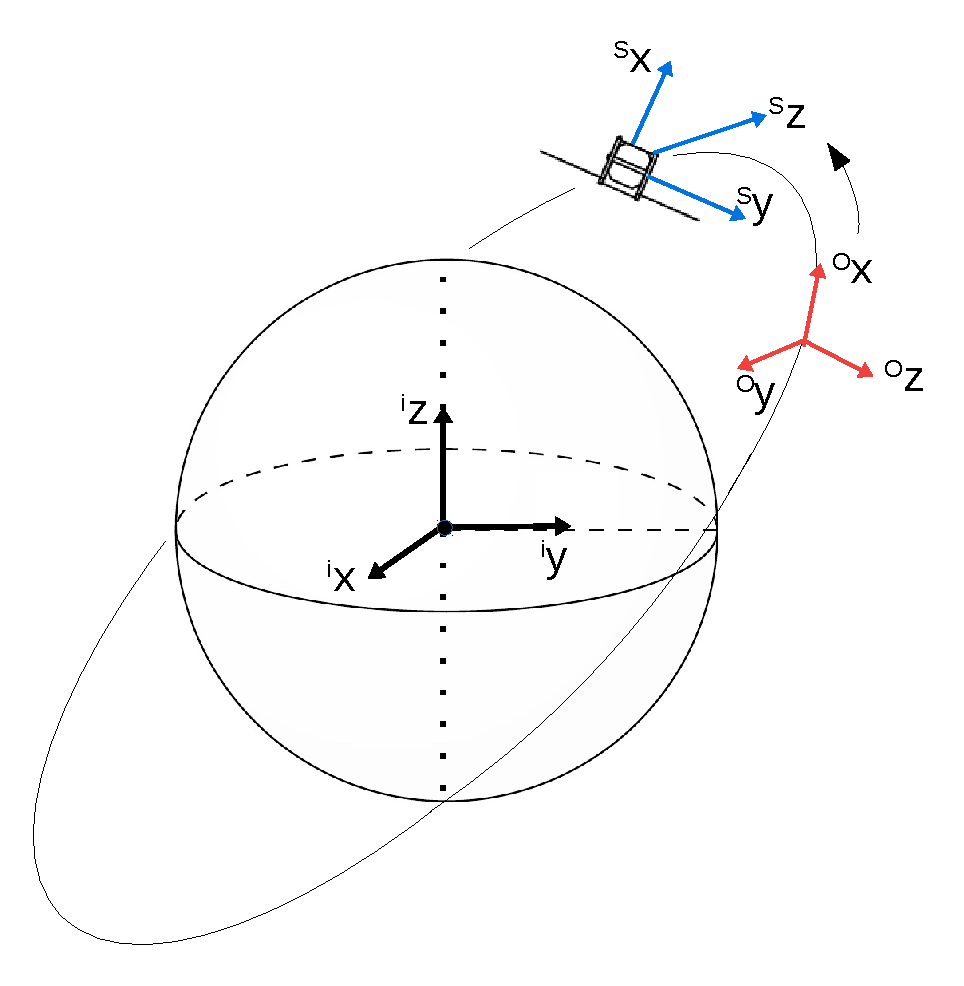
\includegraphics[width=140mm]{figures/frame.pdf}	
	\caption{Reference frame axes. Superscripts: i - ECI, o - Orbital, s - Satellite Body Frame \cite{our_report}.}
	\label{fig:frames}
\end{figure}

\subsubsection{Earth Centered Inertial Frame (ECI)}
Earth is rotating and is orbiting the Sun, it accelerates in the direction of the Sun's center of mass, the Sun is orbiting the center of the Milky Way, etc. Thus there is no frame fixed to Earth's center that is an inertial frame \textit{per definitionem}. But in the case of earth orbiting satellites, there exists a coordinate system attached to Earth's center that out of practical considerations can be treated as one, the Earth Centered Inertial Frame (ECI).
As the name suggests, the origin of the coordinate system is the center of earth. Inertial means that the frame doesn't rotate, the direction of stars remain the same. 
ECI is a cartesian coordinate system. Its $^iz$ vector points in the direction of the northern axis of rotation, while the $^ix$ axis towards the vernal equinox. The $^iy$ axis completes the triad of the right-handed Cartesian coordinate system.


\nomenclature[T]{\textbf{Vernal Equinox}}{The vernal equinox is the vector pointing towards the Sun's center during the equinox (20th of March in 2018). The $x$ vector also keeps its direction relative to the stars.}


\subsubsection{Earth Centered Earth Fixed Frame (ECEF)}

ECEF, similarly to ECI is centered at the Earth's origin. Its $z$ vector points towards the north parallel to the rotational axis. Its $x$ axis points at $0\deg$ latitude and $0\deg$ longitude on the Earth's surface, thus following Earth's rotation. This makes ECEF non-inertial. $y$ axis completes the right-handed triad.

\subsubsection{Orbital Frame}

The Orbital Frame is centered at the center of mass of the satellite. The $^oz$ axis points towards the center of Earth, $^ox$ points in the direction of the satellite's velocity, while $^oy$ is the normal vector for the orbital plane. The 3 axes make up an orthogonal triad.

\nomenclature[T]{\textbf{Nadir}}{The axis pointing towards Earth's center of mass}

\subsubsection{Satellite Body Reference Frame (SBRF)}

Body-fixed frames are attached to the satellite's body, but the orientation of the frame in relation to the body is arbitrary. Due to practical considerations the axes of the SBRF are chosen to line up with the principal axes of inertia of the body.

\chapter{System Description}\label{chap:systemDescribtion}

\section{Reaction Wheels}

One method of controlling a spacecraft's attitude is by using either reaction or momentum wheels attached to the spacecraft's body. By controlling the wheel's angular velocity using a motor, the amount of angular momentum stored in the wheel can be controlled. If there are no external forces involved, the sum of angular momentum in the system made up by the spacecraft's body and the reaction wheels is constant. This means that by increasing the angular velocity of the wheels, the satellite body's angular momentum can be reduced. This angular momentum transfer can be used to control the attitude of the satellite. If the goal is to change the angular momentum of the whole satellite, actuators that have external interaction should be used, such as magnetorquers or solar sails.

The difference between momentum and reaction wheels is that the nominal angular velocity of momentum wheels is high in order to store angular momentum, and in the case of reaction wheels, low. Many momentum wheels still turn at an angular velocity larger than zero in order to avoid static friction in the bearings. Reaction wheels usually make up only a small fraction of a satellite's weight. They rely on being able to run at high speeds, making their angular momentum significant. The small weight ratio makes precise controlling easier.


%One design consideration for reaction wheels is maximizing moment of inertia for unit weight. This is done by distributing most of the material near the outskirts of the wheel. There is a trade-off between having most of the mass at the outskirts and durability at high angular velocities. 


Reaction wheels have an angular velocity limitation. This means that if a reaction wheel reaches its maximum angular velocity, it can no longer generate a torque on the satellite's body in one direction. In this scenario the system's controllability decreases, thus it should be avoided. An angular momentum unloading strategy should be designed to avoid it. Instead of returning the angular momentum to the satellite's body, unloading the angular momentum through other methods is preferred. Magnetorquers can be used for such purposes.

Moving parts are usually prone to failures. Reaction wheels are expected to run at high angular velocities, which wears down the lubrication and the bearings. Reaction wheels equipped with active magnetic bearings are in development \cite{MagneticReactWheel}. These can eliminate friction from the system and by controlling the bearing, can even reduce micro-vibrations, increasing the durability of the system. AAUSAT-II itself however uses mechanical wheel bearings.

\subsection{Reaction Wheel Configuration}

There have been studies on what is the best configuration of redundant reaction wheels. The optimal configuration can of course depend on the requirements. In some configurations the   Minimizing energy consumption is normally the goal in deciding on a configuration. Ismail et al. \cite{ReactionWheelConfigSim} investigated several configurations by running simulations with the configuration being the only difference.

evenly distributed

angular acceleration demand \cite{ReactionWheelConfigSim} \cite{reactionWheelConfigThesis}

gps orientation, Earth station

Tetrahedron configuration can output twice as much force along an axis as one wheel can produce along its own axis.

\subsubsection{Transformation Between Body \& Reaction Wheel Space}

The main attitude controller sends torque demands to the actuators. The torque demand distributed to the reaction wheels have to be converted to torques parallel to reaction wheel axes, in order for the motor controllers to function. Transformation from reaction wheel space to body frame is quite intuitive. Knowing the orientation of each motor axis and the corresponding motor torque

\begin{equation}
N_{rw} = A N_{motor} = \begin{bmatrix}
Axis_{1}       & Axis_{2}  & Axis_{3}  & Axis_{4} 
\end{bmatrix} N_{motor}
\end{equation}

\begin{equation}
A N_{motor}  = 
\begin{bmatrix}
\cos(19.47)       & -\cos(19.47) \cos(60)  &  -\cos(19.47) \cos(60)  & 0 \\
0       & \cos(19.47) \cos(30)  &  -\cos(19.47) \cos(30)  & 0 \\
-\sin(19.47)       & -\sin(19.47)   &  -\sin(19.47)   & 1
\end{bmatrix} N_{motor}
\end{equation}

Since $A$ is a $ 4 \times 3 $ matrix, a pseudo inverse has to be used when reordering the equation.

\begin{equation}
N_{motor} = A ^\dagger N_{rw}   =  A^T  (A A ^T)^{-1} N_{rw}
\end{equation}

\nomenclature{$N_{motor$}}{$4\times1 vector where each entry represents the torque of each reaction wheel motor. $}

\cite[equation 18.41-42]{SADC}
\cite{reactionWheelConfigThesis}

\begin{equation}
h_{rot} = A\left[ h_1, h_2, h_3, h_4 \right]^T
\end{equation}

\begin{equation}
N = A^R \textbf{$N_rw$} + k\left(1,-1,-1,1\right)
\end{equation}

\todo{revise 2nd part}

The torque demand for the satellite's body

\subsubsection{Reconfiguration}

Fault isolation for the redundant reaction wheel configuration can be done by detecting which is the reaction wheel where the fault occurred and shutting it off and redistributing the torques to the rest of the reaction wheels. This reconfiguration can be represented by swapping the corresponding faulty columns to zero vectors. For example, if a fault occurs in the 3rd reaction wheel:

\begin{equation}
A_{f3} = \begin{bmatrix}
Axis_{1}       & Axis_{2}  & 0  & Axis_{4} 
\end{bmatrix}
\end{equation}

The pseudo inverse is calculated in the same manner as presented in ... 

\section*{Magnetorquer model}
\nomenclature[Sncoil]{$n_{coil}$}{The number of windings of the coil}
\nomenclature[SIcoil]{$I_{coil}$}{The electric current flowing through the coil}
\nomenclature[SAcoil]{$\vec A_{coil}$}{The vector perpendicular to the cross-sectional area of the magnetorquer}
\nomenclature[Sm]{$\vec m_{mt}$}{The magnetic dipole moment}

Since the primary actuators for the satellite are chosen to be reaction wheels, four magnetorquer will be used for desaturation of the reaction wheels.  

Having a solenoid onboard of the satellite, referred as a magnetorquer through which the current could be controlled and hence the dipole moment.

The interaction of the dipole with the magnetic field of the Earth will result in a torque that will be perpendicular to the magnetic field vector according to the following equation \cite{SADC}:
\begin{flalign}
   \vec N_{mt} = \vec m_{mt} \times \vec B
	\label{eq:NT}
\end{flalign} 
where $\vec N$ is the torque produce by the magnetorquer and will be the torque that will influence the satellite dynamics, $\vec B$ is the vector of the magnetic field of the Earth and $\vec m_{mt} $ is the magnetic dipole moment generated by the magnetorquer.

The magnetic moment $\vec m_{mt}$ is given by \cite{MagMom}:
\begin{flalign}
	\vec m_{mt} = n_{coil} \ I_{coil} \ \vec A_{coil}
	\label{eq:mm}
\end{flalign} 
where $n_{coil}$ is the windings of the coil, $I_{coil}$ is the electric current on the coil and $\vec A_{coil}$ is the vector perpendicular to the cross-sectional area of the magnetorquer.

Using \ref{eq:NT} and \ref{eq:mm} and taking the magnitude, the applied torque on the satellite is \cite{SJ}:
\begin{flalign}
	\vec N_{mt} = n_{coil} \ \rvert I_{coil}\rvert \ \rvert \vec A_{coil}\rvert \ |\vec B| \sin (\theta)
	\label{eq:ft}
\end{flalign} 
where $\sin (\theta)$ is the angle between the plane $A_{coil}$ and the magnetic field vector $\vec B$.

Furthermore, the resistance of the magnetorqer which is a function of the temperature of the coil given as an input, can be computed as
\begin{flalign}
R_{mt} = \dfrac{nC  \rho_{mt} }{A_{wire}} = \dfrac{nC \rho_0(1+\alpha_0(T_{mt} - T_0))}{A_{wire}}
\label{eq:rt}
\end{flalign} 
where \\
$R_{mt}$ is the resistance of the magnetorquer \\
$n$ is the number of windings \\ 
$C$ is the wire circumference  \\
$A_{wire}$ is the wire cross-sectional area  \\
$\rho_0$ is the resistivity of copper  \\
$\alpha_0$ is the coefficient of resistivity temperature   \\
$T_{mt}$ is the temperature given as an input   \\
$T_0$ is the resistivity base temperature  

Using the computed resistance the current is found by dividing the voltage by the resistance of the magnetorquer. Next, in order to find the magnetic moment $m$, the current is multiplied by the number of windings and the area of the wire. For finding the torque that acts on the satellite, the magnetic moment is multiplied by the coil normal and a cross-product is used between this multiplication and the magnetic field of the Earth.

In order to find what voltage to output for having a certain amount of torque, a gain between voltage and magnetic moment is found. For the coil model, the control signal is the voltage. Therefore, translating the magnetic moment demand to voltage is found as follows:
\begin{flalign}
\frac{\vec m_{mt}}{v} = \frac{n_{coil} \vec A_{coil} \vec I_{coil}}{R_{mt}} \mathcal {K}
	\label{eq:gain}
\end{flalign} 
\begin{flalign}
 \mathcal{K} = \frac{\vec m_{mt} R_{mt} }{ n_{coil}  \vec A_{coil} \vec I_{coil} v}
	\label{eq:gainn}
\end{flalign} 
where \\
$v$ is the voltage \\
$\mathcal {K}$ is the gain

The voltage can be found using the following transfer function:
\begin{flalign}
	\frac{I_{coil}}{v} = \frac{1}{R_{mt}}
	\label{eq:voltage}
\end{flalign} 

where the voltage is found to be $1.25 V$

Given a current $I$ going through a coil, the interest is to find the magnetic field $B$ at a certain point located distance $r$ from the coil. Finding an estimate of the magnetic field at any point will give the possibility to change the location of the magnetometers around. For computing the magnetic field in the center of a rectangular coil, the law of Biot-Savart is used \cite{SJ}:
\begin{flalign}
	d\vec B = \frac{\mu_0 I}{4 \pi}  \frac{d \vec s \times \hat{\vec r}}{r^2}
	\label{eq:BS}
\end{flalign} 
where \\
$\vec B$ is the magnetic field \\
$\mu_0$ is a constant called permeability of free space and is equal with $4\pi \times 10^{-7}  \ Tm/A$ \\
$I$ is the current \\
$d \vec s $ is a length element in the direction of current \\
$\hat{\vec r}$ is the direction from $d \vec s$ to a particular position \\
$r$ is the distance from $d \vec s$ to a particular position

The magnetic field $B$ at any point is directly proportional to the current $I$ that is crossing the coil. The magnetic field generated by the current from equation \ref{eq:BS} is just a small length element $d \vec s$ of the coil. For finding the total magnetic field, all small elements need to be summed up and for this the magnetic field $B$ have to be evaluated by integrating equation \ref{eq:BS}.

The design of the magnetorquer is described in appendix \ref{chap:F}.


\section{Desaturation}

The reaction wheel DC motors and bearings have a limited angular velocity range they can operate in. When the velocity reaches the limit, the motor can no longer accelerate the wheel further in one direction, thus reducing controllability. To avoid this, the wheel velocity should be kept near zero. Usually the speed is above zero to avoid static friction in the bearings. Decreasing the reaction wheel speed by transferring its angular momentum is called desaturation.

Reaction wheels are used to control the attitude of the satellite by transferring its angular momentum. Transferring the angular momentum back to the satellite body would be counterproductive, it should be discarded in a different way. Magnetorquers are ideal for desaturation since they can interact with the earth's magnetic field and are able to transfer angular momentum of the satellite body to earth. Since the earth's magnetic field is quite weak, the torque produced by magnetorquers are small compared to the torque of the reaction wheels. Reaction wheels can be used for fast attitude control while magnetorquers are good for gradually desaturating the reaction wheels. The angular momentum transfer happens through the satellite's body, but with the right control scheme the desaturation can be  completely decoupled from attitude control.

Trégouët et al. \cite{DesatTregouet} developed a cascaded control method for reaction wheel desaturation. The method is a revised version of the so-called cross-product control law. It changes the magnetorquers' magnetic field based on the difference between the angular momentum of the reaction wheels and their reference angular momentum.

\begin{equation}
\vec{\tau_m} = -\frac{\underline{\tilde{b}}^\times(t)}{|\vec{\tilde{b}}(t) |^2} k_p\left(\vec{h_{rw}} - \vec{h_{ref}} \right)
\end{equation}

where  \todo{add the notations to nomenclature}

Momentum dumping and attitude control can potentially be opposing goals, since attitude control changes the reaction wheel velocity to produce the required torque, while the desaturator tries to keep the angular velocity close to the reference. The quasi-cascaded structure of the desaturation control law includes the magnetorquer as the upper subsystem which outputs the rate of change of the total angular momentum of the system \ref{fig:CascadeDesat}. The lower subsystem includes the attitude dynamics and the reaction wheel controller. The problem is that there's a feedback involved from the lower subsystem to the upper one, making $\dot{h}_t$ dependent on the attitude parameters. This means that desaturating the wheels can affect the attitude control loop. Since attitude control is more crucial than desaturation, the reverse would be desirable.  By reversing the ordering of the cascade, the interference can be eliminated. It is done by applying input allocation, i.e. "suitably assigning the low level actuators' input, based on a higher level control effort requested by the control system" \cite{JOHANSEN20131087}. From the point of view of the desaturation controller, the control goal is to keep the reaction wheels' angular velocity as close to the reference velocity as possible. Since the desaturation control is decoupled from attitude control, it can achieve its desaturation control goal regardless of the attitude control law.




\begin{figure}[h]
	\centering
	\begin{tabular}{@{}c@{\hspace{.5cm}}c@{}}
		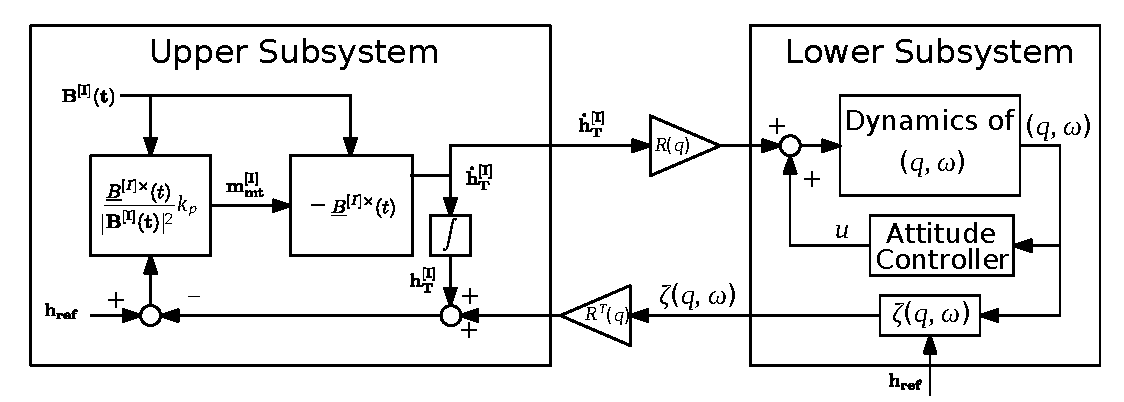
\includegraphics[page=1,width=1\textwidth]{quasiCascadeDesat.pdf}
	\end{tabular}
	\caption{Quasi cascaded desaturation control scheme \cite[Fig. 2.]{DesatTregouet}}
	\label{fig:quasiCascadeDesat}
\end{figure}

According to equation \todo{ref eq in modelling}

\begin{equation}
\underline{I}_{s}\vec{\dot{\omega}} + \underline{\omega}^\times\underline{I}_{s}\vec{\omega} = -\vec{\dot{h}}_{rw} -  \underline{\omega}^\times \vec{{h}}_{rw} + \vec{N_{mt}}  + \vec{N_{dist}} = \vec{u} 
\end{equation}

\begin{equation}
\vec{\tau_m}^{[I]} = -\frac{\underline{\tilde{b}}^\times(t)}{|\vec{\tilde{b}}(t) |^2} k_p\left(\vec{h_{rw}}^{[I]} - \underline{R}^T(\vec{q})\vec{h_{ref}} \right)
\end{equation}

\todo{make it a system of equations}

%\begin{equation}
%\dot{x}_c = 0, (\vec{q},\vec{\omega},x_c) \in C\
%\end{equation}
%
%\begin{equation}
%x_c^+ = -x_c, (\vec{q},\vec{\omega},x_c) \in D\
%\end{equation}
%
%\begin{equation}
%\vec{u} = -c x_c \epsilon -K_\omega \vec{\omega}
%\end{equation}
%
%\begin{equation}
%C:= \left\lbrace (\vec{q},\vec{\omega},x_c) \in \mathbb{S}^3 \times \mathbb{R}^3 \times \left\lbrace -1,1 \right\rbrace : x_c\eta \geq -\delta \right\rbrace 
%\end{equation}
%
%\begin{equation}
%D:= \left\lbrace (\vec{q},\vec{\omega},x_c) \in \mathbb{S}^3 \times \mathbb{R}^3 \times \left\lbrace -1,1 \right\rbrace : x_c\eta \leq -\delta \right\rbrace 
%\end{equation}

as shown in \ref{eq:finaleq}
\begin{flalign}
\vec{ ^s_i\dot q(t)}  = \dfrac{1}{2} \underline \Omega \  \vec{^s_i q(t)}
\end{flalign} 

\[
\begin{array}{l}

\dot{x}_c = 0, (\vec{q},\vec{\omega},x_c) \in C\ \\ 
x_c^+ = -x_c, (\vec{q},\vec{\omega},x_c) \in D\ \\ 
\vec{u} = -c x_c \epsilon -K_\omega \vec{\omega} \\
C:= \left\lbrace (\vec{q},\vec{\omega},x_c) \in \mathbb{S}^3 \times \mathbb{R}^3 \times \left\lbrace -1,1 \right\rbrace : x_c\eta \geq -\delta \right\rbrace  \\

D:= \left\lbrace (\vec{q},\vec{\omega},x_c) \in \mathbb{S}^3 \times \mathbb{R}^3 \times \left\lbrace -1,1 \right\rbrace : x_c\eta \leq -\delta \right\rbrace 
\end{array}
\]

\todo{this attitude controller should be down as one of the possible attitude controllers - "Satellite angular momentum removal utilizing the earth’s magnetic field" article}

\begin{figure}[h]
	\centering
	\begin{tabular}{@{}c@{\hspace{.5cm}}c@{}}
		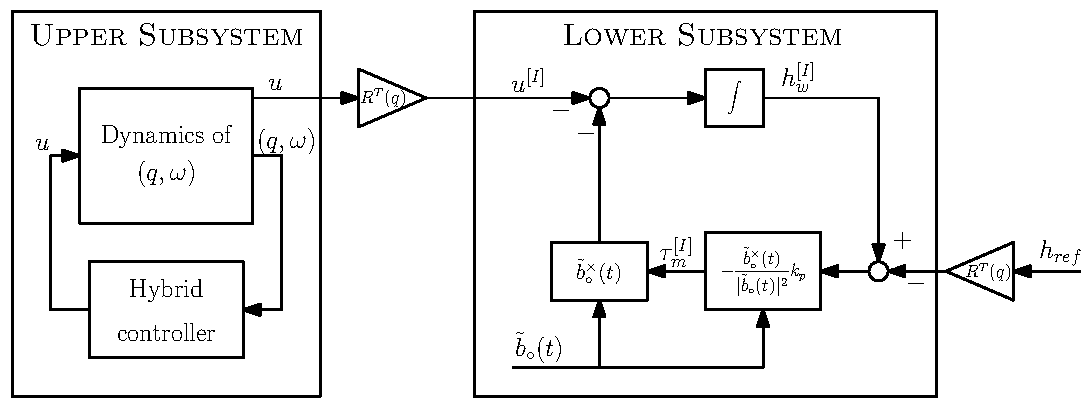
\includegraphics[page=1,width=1\textwidth]{cascadeDesat.pdf}
	\end{tabular}
	\caption{Cascaded desaturation control scheme  \cite[Fig. 4.]{DesatTregouet}}
	\label{fig:CascadeDesat}
\end{figure}

The derived equations that can be implemented in simulation:

\begin{equation}
\vec{\dot{\omega}} = \underline{I}_{s}^{-1}\left( \vec{u} -  \underline{\omega}^\times\underline{I}_{s}\vec{\omega}  \right) 
\end{equation}

\begin{equation}
\vec{\dot{h}}_{rw} =  -  \underline{\omega}^\times \vec{{h}}_{rw} + \vec{N_{mt}}  + \vec{N_{dist}} - \vec{u} 
\end{equation}

\todo{body-fixed frame
	Static input allocation
	global asymptotic stability}

\cite{DesatYang}
\chapter{Requirements}\label{chap:requirements}
Based on the use-case introduced and the available system a set of requirements are formulated.
%
\subsection*{System requirements}
%
\begin{enumerate}
	\item \textbf{The satellite should reconfig scheme control .}
	
	desc
	
	\item \textbf{The satellite should detect the faults .}
	
	desc
	
\end{enumerate}

The satellite shall detect certain actuator faults.

It should be able to reconfigure the control scheme in order to handle faults. 



MUST is equivalent to REQUIRED and SHALL indicating that the definition is an absolute requirement.

MUST NOT is equivalent to SHALL NOT and indicates that it is an absolute prohibition of the specs.

SHOULD is equivalent to RECOMMENDED means that there are valid reasons to ignore a particular requirement, but the implications need to be weighed.

SHOULD NOT and NOT RECOMMENDED means that a particular behavior may be acceptable or useful, but again, the implications need to be weighed.

MAY means OPTIONAL and that the requirement is truly optional. Interoperability with different systems that may or may not implement an optional requirement must be done.

$\dot \omega $
\chapter{Angle control between satellites}

\chapter{Fault  analysis}
\textit{In this chapter, probable faults in the system are examined using a Failure Mode and Effects Analysis (FMEA). Next, in order to find how probable a fault will happen and the effect of it, the severity and occurrance (SO) of faults is analyzed. It was decided that the fault analysis will be carry out only for the actuators (magnetorquers and momentum wheels).}

A fault in a system can be seen as a sudden shift in the system functionality, nevertheless, it might not mean a total shutdown of the system. One way to see it is as a disturbance in the system, that might cause performance loss or serious deterioration to the system. On the other hand, a failure can be understood as a total shutdown of the system component. 

In \figref{fig:1} a fault tolerant system is described, which contains an autonomous supervisor that has the ability to switch between various controllers taking into account the type of fault that a component has. The spacecraft block illustrated in the picture is composed of a plant, actuators and sensors and is monitored by the fault detection and isolation (FDI) system, which include detectors that will feed informations to the supervisor in the eventuality of a fault. Based on the information received, the supervisor will establish if a fault occurred or not and in case of a fault the effectors will handle it. Figure \ref{fig:2} shows the procedure of how faults are handled with varius methods.

\begin{table}[H]
	\begin{minipage}[b]{0.49\linewidth}
		\centering
		\begin{figure}[H]
			\centering
			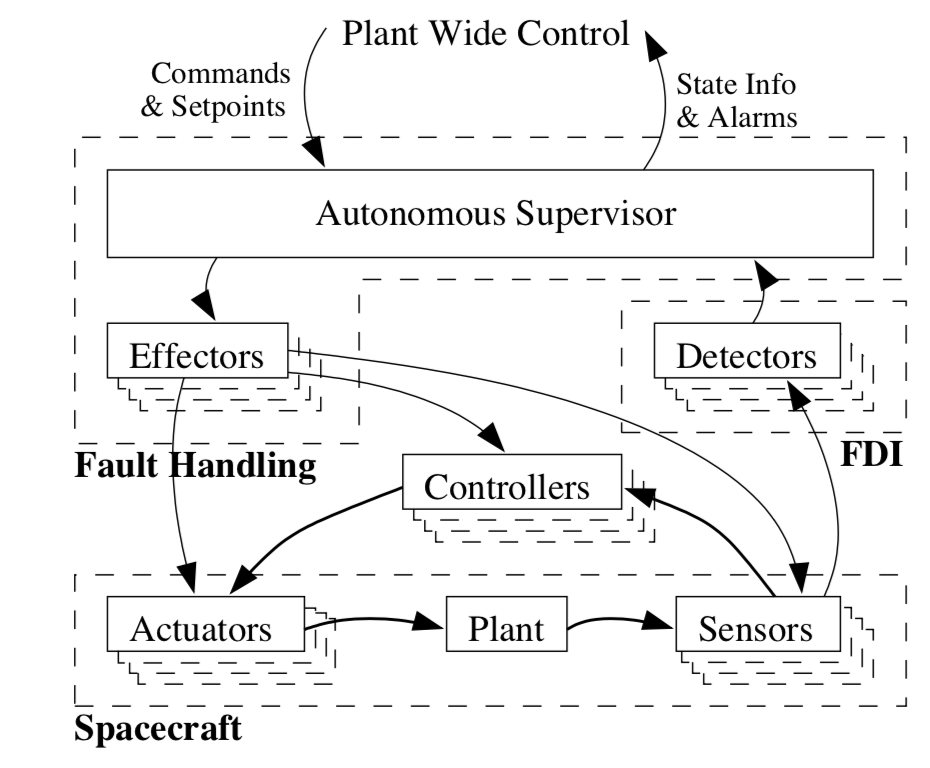
\includegraphics[width=1\linewidth]{figures/FTC}
			\caption{Fault tolerant system architecture [ref jesper article}
			\label{fig:1}
		\end{figure}
	\end{minipage}\hfill
	\begin{minipage}[b]{0.49\linewidth}
		\centering
		\begin{figure}[H]
			\centering
			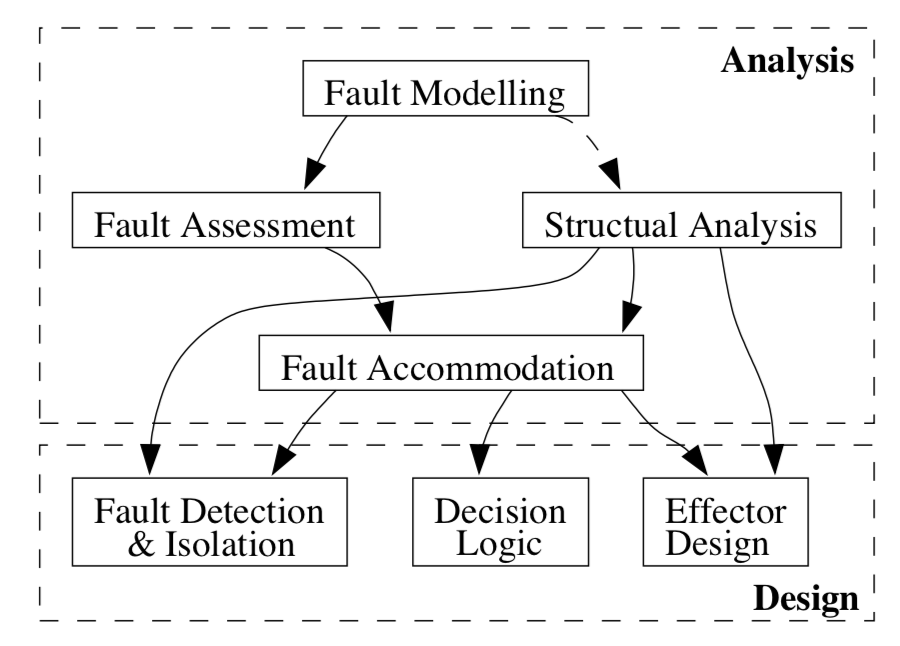
\includegraphics[width=1\linewidth]{figures/FTC_2}
			\caption{ }
			\label{fig:2}
		\end{figure}
	\end{minipage}
\end{table}

\subsection{Failure Mode and Effects Analysis}
A FMEA analysis which is a bottom-up analysis method is performed for the components of the satellite. The main goal of FMEA is to identify possible faults and their effect on components. In order to evaluate how faults are propagated through the system, a FMEA scheme is constructed.
Another aspect of FMEA analysis is that, the severity of a fault can be determined, which will offer the opportunity to prioritize the faults by severity and in this way focus on the important faults.

In order to control the attitude of the satellite, two types of actuators are used: magnetorquers and momentum wheels. Potential faults are gather into a table which describes the effect and cause, while the satellite is orbiting.
\subsubsection{Magnetorquers}

\begin{table}[H]
	\centering
	\label{my-label}
	\begin{tabular}{|l|l|l|}
		\hline
		\multicolumn{3}{|c|}{\textit{\textbf{Magnetorquers}}}                                          \\ \hline
		\multicolumn{3}{|c|}{Produces a magnetic field that interacts with Earth's magnetic field}                     \\ \hline
		\textbf{Reference} & \textbf{Failure Effect} & \textbf{Failure Cause}                          \\ \hline
		MT1                & Low magnetic field  & \begin{tabular}[c]{@{}l@{}}- Broken wire or bad soldering\\ - Component burned\end{tabular} \\ \hline
		MT2                & Maximum magnetic field power  & Short circuit to the power voltage   \\ \hline
		MT3                & Wrong direction of the magnetic field & \begin{tabular}[c]{@{}l@{}}- Misalignment of the magnetorquer\\ - Short circuit of some parts of the \\ torquer to the power voltage \end{tabular} \\ \hline
		MT4                & Wrong  power of the magnetic field                 & Floating supplay voltage                                            \\ \hline
	\end{tabular}
	\caption{Potential faults in the magnetorquers}
\end{table}

\subsubsection{Momentum wheels}
\begin{table}[H]
	\centering
	\label{my-label}
	\begin{tabular}{|l|l|l|}
		\hline
		\multicolumn{3}{|c|}{\textit{\textbf{Momentum wheels}}}                                          \\ \hline
		\multicolumn{3}{|c|}{Produces a torque about the satellite COM in order to rotate it }                     \\ \hline
		\textbf{Reference} & \textbf{Failure Effect} & \textbf{Failure Cause}                          \\ \hline
		MW1                & Faulty orientation & \begin{tabular}[c]{@{}l@{}}- Missing flywheel\\ - Component burned\end{tabular} \\ \hline
		MW2                & -  & Short circuit to the power voltage   \\ \hline
		MW3                & -& \begin{tabular}[c]{@{}l@{}} Short circuit to the ground\\  \end{tabular} \\ \hline
		MW4                & -                & Broken wire or bad soldering                                          \\ \hline
	\end{tabular}
	\caption{Potential faults in the momentum wheels}
\end{table}

\subsubsection{Fault propagation analysis}

\subsection{Fault detection and isolation}

\chapter{Acceptance test} \label{chap:acceptanceTest}

The system is tested to see if it fulfills the requirements put up (\chapref{chap:requirements}).

Nadir pointing capability is tested by turning on the linear attitude controller of a satellite with initial attitude and angular velocity deviating from the reference. After reducing the initial error, the tracking error stays below $1^o$, as shown in figure 9.1.

\begin{figure}[H]
	\centering
	%	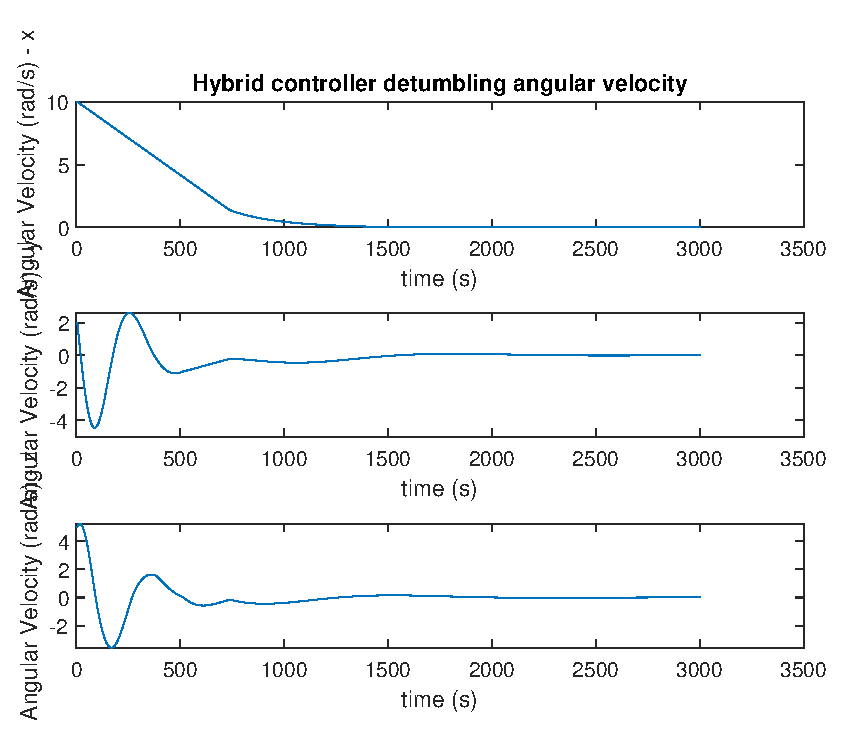
\includegraphics[width=0.7\linewidth]{figures/detumbling3}
	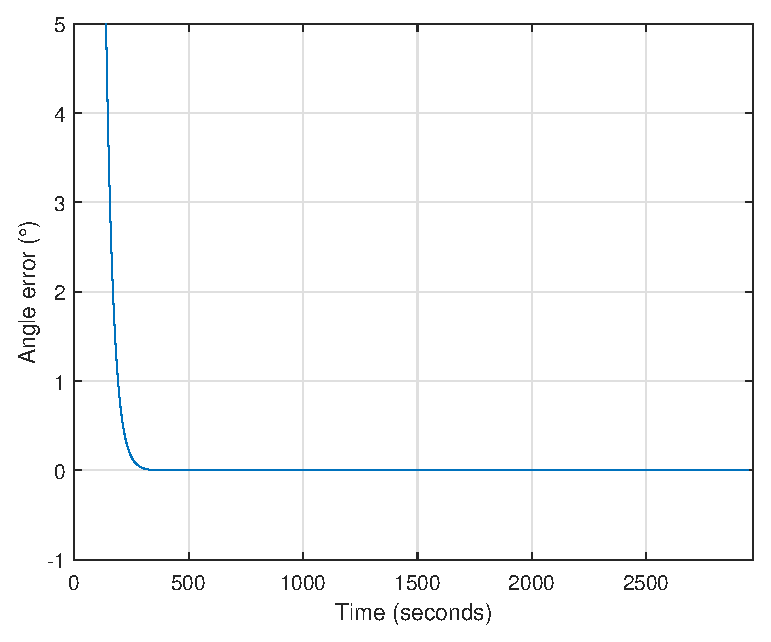
\includegraphics[width=0.7\linewidth]{figures/angle_error}
	\caption{Tracking error during nadir pointing}
	\label{fig:angle_error}
\end{figure}

Earth station tracking is  tested in a scenario where the satellite flies right over the station. This is the closest the satellite in orbit can get to the Earth station, leading to maximum torque demand. The tracking error is kept below  $1^o$, with error peaks appearing during flyover. Figures \ref{fig:angle_error2} and \ref{fig:torque_stationTrack} present the tracking error and torque demand arising during station tracking.

\begin{figure}[H]
	\centering
	%	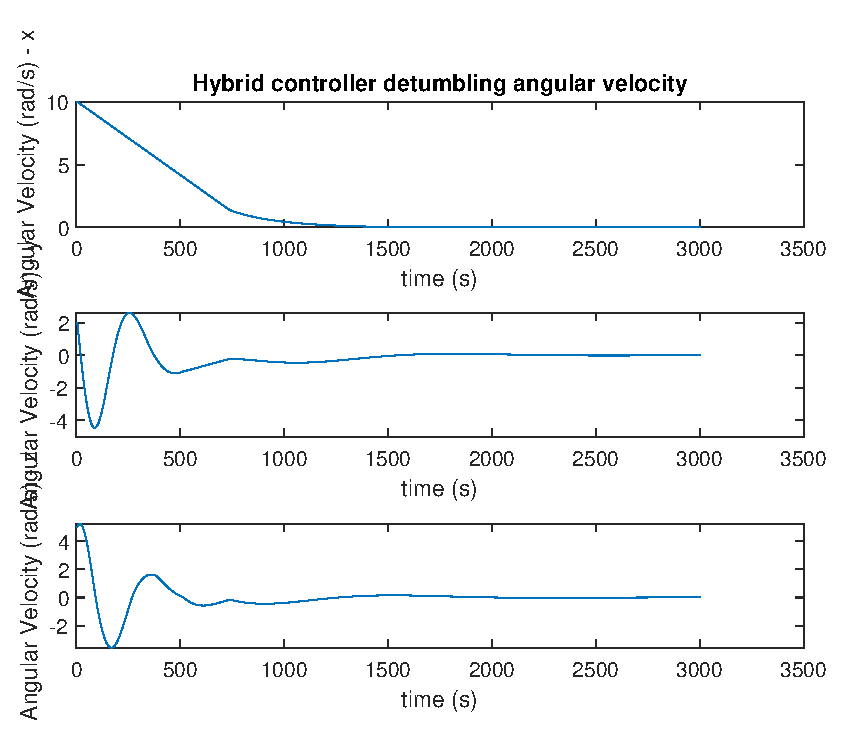
\includegraphics[width=0.7\linewidth]{figures/detumbling3}
	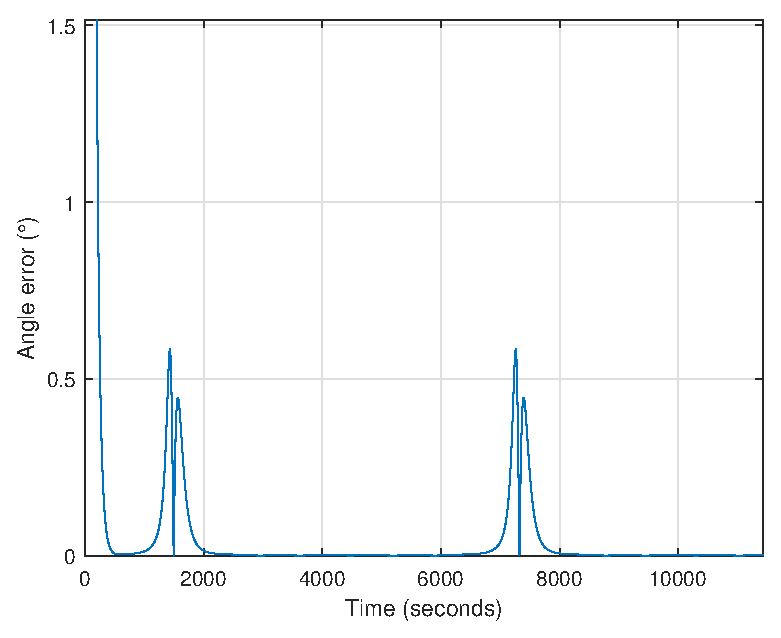
\includegraphics[width=0.7\linewidth]{figures/angle_error_stationTrack}
	\caption{Tracking error during Earth station pointing. The satellite flies over the station.}
	\label{fig:angle_error2}
\end{figure}


\begin{figure}[H]
	\centering
	%	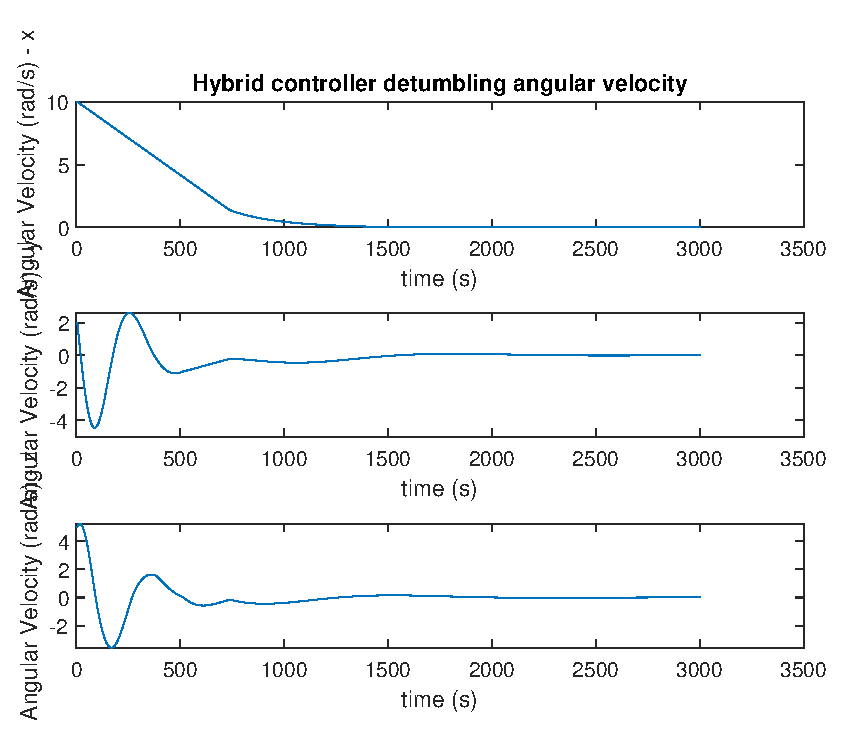
\includegraphics[width=0.7\linewidth]{figures/detumbling3}
	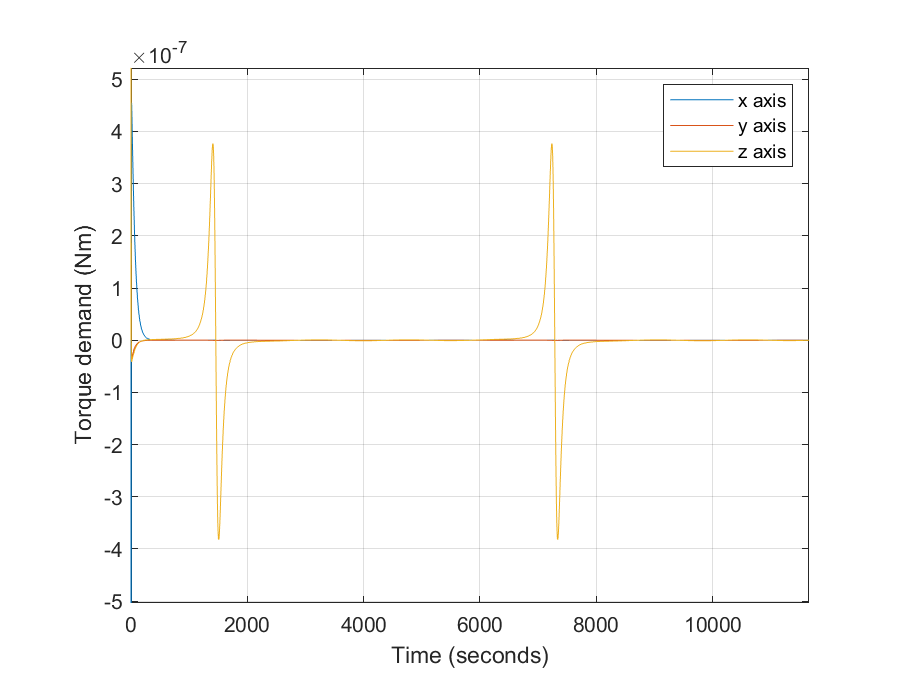
\includegraphics[width=0.7\linewidth]{figures/torque_stationTrack}
	\caption{Torque demand $\vec{u}$ during Earth station pointing. The satellite flies over the station.}
	\label{fig:torque_stationTrack}
\end{figure}

\begin{figure}[H]
	\centering
	%	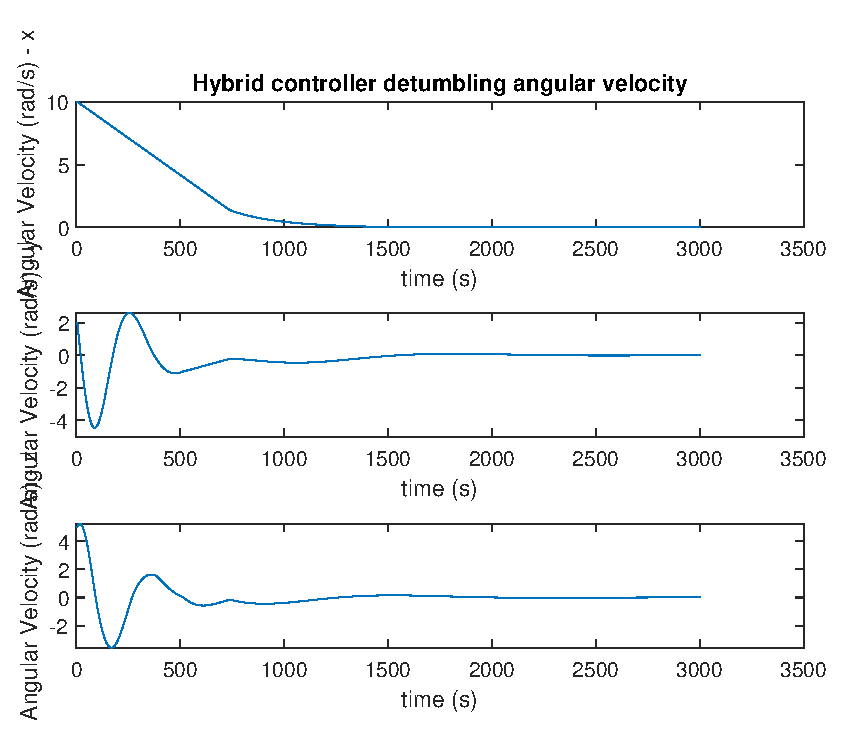
\includegraphics[width=0.7\linewidth]{figures/detumbling3}
	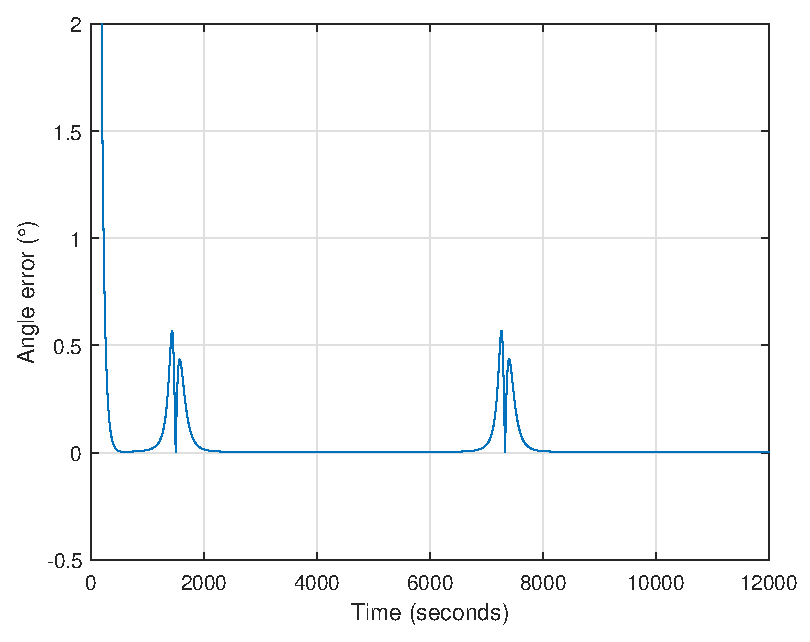
\includegraphics[width=0.7\linewidth]{figures/faultyangerror}
	\caption{Tracking error during Earth station pointing using the linear controller. The satellite flies over the station. The 3rd reaction wheel is faulty and switched off.}
	\label{fig:angle_error2}
\end{figure}


%\subsection{1. The formation shall be able to maintain a given angle within 45$^{\circ}$.}
%The

\chapter{Conclusion}
The overall objective of this project was to consider several satellites flying in formation with the purpose of pointing towards a target. In order to reach this goal, two controllers were designed: one for controlling the angle between satellites using the drag force and another one for attitude control in order to be able to rotate the satellite to the desired orientation.

First, for designing a controller for the angle, the relative dynamics between two satellites are analyzed. Therefore, an LQR controller is implemented to control the angle between two satellites. The simulations showed that the LQR performed properly. Additionally, two algorithms for formation control are designed, a global and distributed algorithm. Both algorithms are working as intended, where the angles between neighbour satellites converged to the desired angle of 45$^{\circ}$, with the mention that in the distributed algorithm case the convergence rate will be slower compared with the global algorithm.

Afterwards, two control methods to obtain the desired orientation of the satellite has been implemented. The first method is a state feedback which is a linear control method. For implementing this controller the equation of motion need to be linearized. The second method is using a non-linear control method called sliding mode control. The results from sliding mode control showed that the error quaternion converged better compared to state feedback control, but in this case, the state feedback is deemed to be more suitable. Besides, the sliding mode convergence is better, but due to the fact that the control law is more complex, the satellite controller will need more computation time. 

In conclusion, some acceptance tests have been made to establish that the requirements accomplished. 


%%% Bibliography %%%
%---------- Appendix Below ----------------------------------------
\appendix
\chapter{Derivation of relative dynamics equations} \label{chap:B}
The vector position from the centre of the Earth to the satellite 1 and the satellite 2 is given by
\begin{flalign}
\vec{p_1} &= R  \vec{\hat{x}} \\
\vec{p_2} &= R  \vec{\hat{x}} + x  \vec{\hat{x}} + y  \vec{\hat{y}}
\end{flalign}
the first time derivative and second time relative of $\vec{p_1}$ and $\vec{p_2}$ is computed:
\begin{flalign*}
\vec{\dot{p}_1} &= \dot{R}  \vec{\hat{x}} + R(\vec{w} \times \vec{\hat{x}}) 
\end{flalign*}
where $\vec{w}$ is the angular velocity vector and $\vec{w} = w  \vec{\hat{z}}$ due to the fact the position of the satellites stay all over the time in the plan $(\vec{\hat{x}},\vec{\hat{y}})$. Therefore, the first time derivative and the second time derivative are given by:
\begin{flalign*}
\\vec{\dot{p}_1} &= \dot{R}  \vec{\hat{x}} + w R  \vec{\hat{y}} \\
\vec{\ddot{p}_1} &= \ddot{R}  \vec{\hat{x}} + w\dot{R}  \vec{\hat{y}} + \dot{w} R  \vec{\hat{y}} + w \dot{R}  \vec{\hat{y}} + wR  (\vec{w} \times \vec{\hat{y}}) \\
&= \ddot{R}  \vec{\hat{x}} + 2w\dot{R}  \vec{\hat{y}} - w^2R  \vec{\hat{x}} \\
\vec{\dot{p}_2} &= \vec{\dot{p}_1} +  \dot{x}  \vec{\hat{x}} + x w  \vec{\hat{y}} + \dot{y}  \vec{\hat{y}} - y w  \vec{\hat{x}} \\
&= \vec{\dot{p}_1} + (\dot{x} - yw)  \vec{\hat{x}} + (xw + \dot{y})  \vec{\hat{y}} \\
\vec{\ddot{p}_2} & = \vec{\ddot{p}_1} + (\ddot{x} - \dot{y}w - y\dot{w})  \vec{\hat{x}} + (\dot{x} - yw) w  \vec{\hat{y}} + (\dot{x}w + x\dot{w} + \ddot{y})  \vec{\hat{y}} - (xw + \dot{y}) w  \vec{\hat{x}} \\
&= \vec{\ddot{p}_1} + (\ddot{x} - 2\dot{y}w - y\dot{w} - xw^2)  \vec{\hat{x}} + (\ddot{y} + 2\dot{x}w + x\dot{w} - yw^2)  \vec{\hat{y}}
\end{flalign*}
Furthermore, The Newton law gives:
\begin{flalign}
	m\vec{\ddot{p}_1} &= \vec{F_{grav,1}} + \vec{F_{drag,1}} + \vec{F_{dist,1}}	\label{eq:l3} \\
	m\vec{\ddot{p}_2} &= \vec{F_{grav,2}} + \vec{F_{drag,2}} + \vec{F_{dist,2}} 	\label{eq:l4} \\
	\Rightarrow \vec{\ddot{p}_2} - \vec{\ddot{p}_2} &= \frac{1}{m}(\Delta \vec{F_{grav}} + \Delta \vec{F_{drag}} + \Delta \vec F_{dist}) 	\label{eq:l5}
\end{flalign}
with m is the mass of both satellites. The gravity is given by the universal law of gravitation:
\begin{flalign*}
\frac{\vec{F_{grav,1}}}{m} &= -G\frac{m_{earth}}{||\vec{R}||^3} \vec{R} \\
\frac{\vec{F_{grav,2}}}{m} &= -G\frac{m_{earth}}{||\vec{R} + \vec{r}||^3} (\vec{R} + \vec{r})
\end{flalign*}
where $\vec{r} = (x,y)$ is the vector from the satellite 1 to the satellite 2. The denominateur can be approximated using:
\begin{flalign*}
||\vec{R} + \vec{r}||^{-3} &= ||\vec{r}|| \\
%||\vec{R} + \vec{r}||^{-3} &= ||(\vec{R} + \vec{r})\cdot(\vec{R} + \vec{r})||^{\frac{-3}{2}} \\
%&= ||\vec{R} \cdot \vec{R} + \vec{r} \cdot \vec{r} + 2\vec{R} \cdot \vec{r}||^{\frac{-3}{2}} \\
%&= R^{-3}||1 + \frac{\vec{r} \cdot \vec{r}}{R^2} + 2\frac{\vec{r} \cdot \vec{R}}{R^2}||^{\frac{-3}{2}}
\end{flalign*}
%Due to the fact the $r << R$, the second term can be neglected and by using the approximation $(1 + x)^q = 1 + qx$ when $x << 1$. The expression can be approximated by:
%\begin{flalign*}
%||\vec{R} + \vec{r}||^{-3} &= R^{-3}(1 - 3\frac{\vec{r} \cdot \vec{R}}{R^2}) \\
%&= R^{-3}(1 - 3\frac{x}{R})
%\end{flalign*} 
and thus, the difference between the gravity force on satellite 2 and the the gravity force on 1 is:
\begin{flalign*}
\vec{F_{grav,2}} - \vec{F_{grav,1}} &\approx -\frac{\mu}{R^3}\vec{r} \\
%\vec{F_{grav,2}} - \vec{F_{grav,1}} &\approx -G \frac{m_{earth}}{R^3} ((1 - 3\frac{x}{R}) (\vec{R} + \vec{r}) - \vec{R}) \\
%&\approx -G \frac{m_{earth}}{R^3} (\vec{r} - 3x \cdot \vec{\hat{x}} + 3 \frac{x}{R} \vec{r}) \\
%&\approx -\frac{\mu}{R^3} (-2x \cdot \vec{\hat{x}} + y \cdot \vec{\hat{y}})
\end{flalign*} 
with $\mu = G  m_{earth}$, The drag force can be modelling be using \eqref{eq:teor}:
\begin{flalign*}
	\vec{F_{drag,1}} &= -u_1 ||\vec{\dot{p}_1}|| \vec{\dot{p}_1}\\
	& = -u_1 ||\vec{\dot{p}_1}|| (\dot{R}  \vec{\hat{x}} + wR  \vec{\hat{y}}) \\
	\vec{F_{drag,2}} &= -u_2 ||\vec{\dot{p}_2}|| \vec{\dot{p}_2} \\
	& = -u_2 ||\vec{\dot{p}_2}|| ((\dot{R} + \dot{x} - yw) \vec{\hat{x}} + (wR + xw + \dot{y})  \vec{\hat{y}})
\end{flalign*}
Therefore, the \eqref{eq:l3} becomes:
\begin{equation}
\left\{
	\begin{aligned}
		&\ddot{R} - w^2R = -\frac{\mu}{R^2} -\frac{u_1}{m} ||\vec{\dot{p}_1}|| \dot{R} + \frac{F_{dist,1,x}}{m} \\
		&2w\dot{R} + \dot{w}R = -\frac{u_1}{m} ||\vec{\dot{p}_1}|| wR + \frac{F_{dist,1,y}}{m}
	\end{aligned}
\right.
\end{equation}
and the \eqref{eq:l5} gives:
\begin{equation}
\left\{
	\begin{aligned}
		& \ddot{x} - 2\dot{y}w - y\dot{w} - xw^2 = -x\frac{\mu}{R^3} + \frac{u_1}{m} ||\vec{\dot{p}_1}|| \dot{R} - \frac{u_2}{m} ||\vec{\dot{p}_2}||(\dot{R} + \dot{x} - yw) + \frac{\Delta F_{dist,x}}{m}\\
		&\ddot{y} + 2\dot{x}w + x\dot{w} - yw^2 = -y\frac{\mu}{R^3} + \frac{u_1}{m}||\vec{\dot{p}_1}||wR - \frac{u_2}{m}||\vec{\dot{p}_2}||(wR + xw + \dot{y}) + \frac{\Delta F_{dist,y}}{m}
	\end{aligned}
\right.
\label{eq:l7}
\end{equation}
The operating point is the position ($x^{*},y^{*}$) of the satellite 2 in the frame of satellite. $x^{*}$ and $y^{*}$ can be computed from \figref{fig:operating_pt}.
\begin{figure}[H]
	\centering
	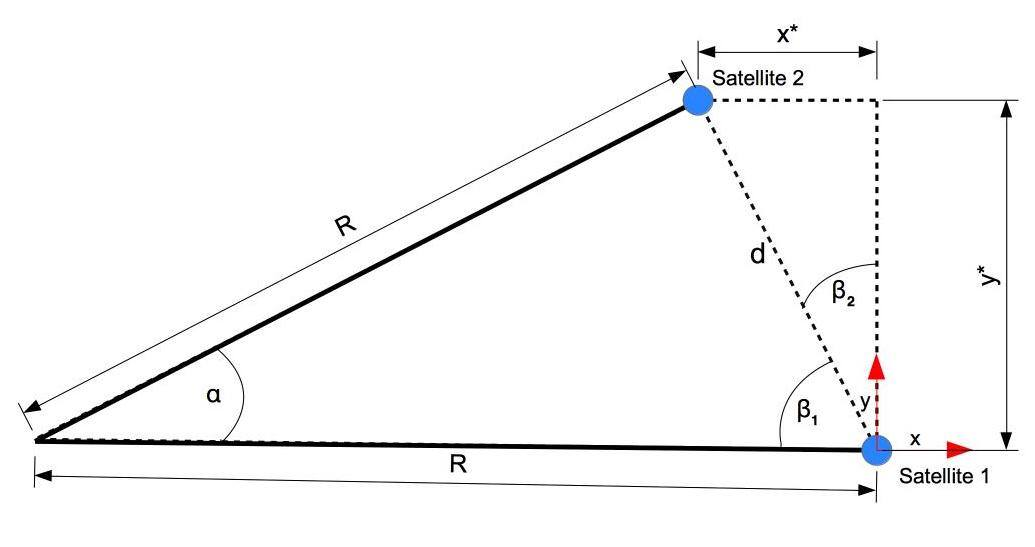
\includegraphics[width=0.75\linewidth]{figures/operating_point}
	\caption{Operating point}
	\label{fig:operating_pt}
\end{figure} 
Using trigonometry relations:
\begin{flalign*}
d &= 2Rsin(\frac{\alpha}{2}) \\
x^{*} &= -dsin(\beta_2) \\
&= -dsin(\frac{\alpha}{2}) \\
&= -2Rsin(\frac{\alpha}{2})^2 \\
y^{*}  &= dcos(\frac{\alpha}{2}) \\
&= 2Rsin(\frac{\alpha}{2})cos(\frac{\alpha}{2}) \\
&= Rsin(\alpha)
\end{flalign*}
with $\alpha$ is the desired angle between satellite and so $\beta_2 = 90^{\circ} - \beta_1 = 90^{\circ} - (90^{\circ} - \frac{\alpha}{2}) = \frac{\alpha}{2}$. Therefore we change the coordinate reference as following:
\begin{flalign*}
x &\Leftarrow x - x^{*}  \\
y &\Leftarrow y - y^{*}  
\end{flalign*}
Thus, the equations \eqref{eq:l7} become:
\begin{equation}
\left\{
\begin{aligned}
	& \ddot{x} - 2\dot{y}w - (y + y^{*})\dot{w} - (x + x^{*})w^2 = \\
	&-(x + x^{*})\frac{\mu}{R^3} + \frac{u_1}{m} ||\vec{\dot{p}_1}|| \dot{R} - \frac{u_2}{m} ||\vec{\dot{p}_2}||(\dot{R} + \dot{x} - (y + y^{*})w) + \frac{\Delta F_{dist,x}}{m}\\
	&\ddot{y} + 2\dot{x}w + (x + x^{*})\dot{w} - (y + y^{*})w^2 =\\
	& -(y + y^{*})\frac{\mu}{R^3} + \frac{u_1}{m}||\vec{\dot{p}_1}||wR - \frac{u_2}{m}||\vec{\dot{p}_2}||(wR + (x + x^{*})w + \dot{y}) + \frac{\Delta F_{dist,y}}{m}
\end{aligned}
\right.
	\label{eq:la1}
\end{equation}
%\subsection{Linearisation of the relative dynamics eqations} \label{sec:C}
%From the equations \eqref{eq:la1} and assuming that the radius is constant and the angular velocity equals to $w = \sqrt{\frac{\mu}{R^3}}$, a linearization of the system can be derived using some approximations. The state is defined as :
%\begin{flalign*}
%	s = [x \ \dot{x} \ y \ \dot{y}]^\mathsf{T}
%\end{flalign*}
%Moreover, the norm of the velocity of both satellite is assumed to be equal and to be constant ($||\vec{\dot{p_1}}|| = ||\vec{\dot{p_2}}|| = C$). Therefore, the nominal system is given by:
%\begin{equation}
%\left\{
%\begin{aligned}
%& \dot{s_1} = s_2 \\
%& \dot{s_2} = 2ws_4 - u_2\frac{y^{*}wC}{m} \\
%& \dot{s_3} = s_4 \\
%& \dot{s_4} = -2ws_2 - (u_2 - u_1)\frac{wRC}{m}
%\label{eq:statespaceassumption}  
%\end{aligned}
%\right.
%\end{equation}
%using the approximation $\dot{x}$, $y << y^{*}$ and $x, x^{*}$, $\frac{\dot{y}}{w} << R$. 
\chapter{Derivation of the satellite equations of motion} \label{chap:C}
This section describes the derivation of the mathematical model of the satellite which contains the dynamic and kinematic model, based on the rigid body dynamics and kinematics.
\subsection{Kinematic equation}
In this subsection, the focus will be on describing the orientation of the satellite. The method used for describing the satellite attitude is quaternion representation. It was decided to choose quaternion representation, because they provide a way to deal with singularities.

The quaternion $\textbf{q}(t)$ is defined as the attitude quaternion of a rigid body at time $t$ with respect to the inertial frame and at time $t+\Delta t$, the quaternion $\textbf{q}(t+\Delta t)$ is defined. The orientation quaternion can be divided into the quaternion at time $t$ and performing a quaternion multiplication with the rotation in the interval $\Delta t$ as follows:
\begin{flalign}
	\vec{ ^s_iq}(t+\Delta{t}) = \vec{ q}(\Delta {t}) \otimes \vec{ ^s_i q}(t) 
	\label{eq:qp}
\end{flalign}
where the orientation quaternion $	\vec{ ^s_iq}(t+\Delta{t}) $ represents the rotation of the spacecraft body frame with respect to the intertial frame

The quaternion at time $\Delta t$ can be express using the triad $u, v, w$, that represent the axis of the spacecraft as:
%
\begin{flalign}
	q_{1}(\Delta {t})  = {e_{u}\sin\frac{\Delta\Phi}{2}}
	\label{eq:q11}
\end{flalign}
%
\begin{flalign}
	q_{2}(\Delta {t}) = {e_{v}\sin\frac{\Delta\Phi}{2}}
	\label{eq:q2}
\end{flalign}
%
\begin{flalign}
	q_{3} (\Delta {t})= {e_{w}\sin\frac{\Delta\Phi}{2}}
	\label{eq:q3}
\end{flalign}
%
\begin{flalign}
	q_{4}(\Delta {t}) = {\cos\frac{\Delta\Phi}{2}}
	\label{eq:q4}
\end{flalign}
where $\Delta \Phi$ is the rotation at time $\Delta t$ and $e_u,e_v, e_w$ are the components along the triad $u, v, w$ at time $\Delta t$.

Using equation \ref{eq:q11} and equation \ref{eq:q4} and insert them into equation \ref{eq:qp} which yields:
\begin{flalign}
	\vec{ ^s_i q}(t+\Delta{t})
	= 
	\left\{\cos\frac{\Delta\Phi}{2} \underline I_{(4\times4)}+\sin\frac{\Delta\Phi}{2}
	\begin{bmatrix}
		0 &e_{z}&-e_{y}&e_{x} \\
		-e_{z}&0&e_{x}&e_{y}  \\ 
		e_{y}&-e_{x}&0&e_{z} \\
		-e_{x} &e_{y}&-e_{z}&0
	\end{bmatrix} 
	\right \} \vec{ ^s_i q}(t)
	\label{eq:quatm}
\end{flalign}  
%
where $\underline I$ is the identity matrix with the dimensions of $4\times4$.

In order to turn equation \ref{eq:quatm} into a differential equation, a small angle approximation it is used: 
\begin{flalign}
	&\Delta \phi = \omega \ \Delta t \\
	&\cos\frac{\Delta\Phi}{2} \approx 1 \\	
	&\sin\frac{\Delta\Phi}{2} \approx \frac{\omega \Delta t }{2} \\
	\label{eq:aprox}
\end{flalign} 
After using the approximation and substitute the terms into \ref{eq:quatm}, the following equation is obtained:
\begin{flalign}
	\vec{^s_i q(t+\Delta{t})} \approx \left[1 + \frac{1}{2} \underline \Omega \Delta(t)\right]\vec{^s_i q(t)}
	\label{eq:quatfinal}
\end{flalign} 
where $\underline \Omega$ is the skew symmetric matrix written in form:
\begin{flalign}
	\underline \Omega
	= 
	\begin{bmatrix}
		0& \omega_{w}& - \omega_{v}& \omega_{u} \\
		-\omega_{w}& 0&\omega_{u}& \omega_{v}  \\ 
		\omega_{v}& -\omega_{u}&0& \omega_{w} \\
		-\omega_{u}& -\omega_{v}& -\omega_{w}&0
	\end{bmatrix} 
	\label{eq:sm}
\end{flalign}
where the terms $\omega_u, \omega_v, \omega_w$ are the angular velocities componets.

The rate of change in the orientation of the spacecraft $\vec{^s_i q(t)}$  can be found:
\begin{flalign}
	\vec{ ^s_i\dot q(t)} = \lim_{\Delta t\to 0} \frac{\vec q(t+\Delta t) - \vec q(t)}{\Delta t} = \dfrac{1}{2} \underline \Omega \  \vec{^s_i q(t)}
	\label{eq:finaleq}
\end{flalign} 

\subsection{ Dynamic equation}
The satellite dynamics are described using Euler's equation of motion and Newton's laws of motion. 
Using Euler's equation of motion, the relation between the change in angular momentum and the torques that affect the satellite is given as follows:
\begin{flalign}
	\vec{ \dot h} = \vec{N_{ext}} =  \vec{N_{mt}}+ \vec{N_{dist}}
	\label{eq:ec2}
\end{flalign} 
where $h$ is the angular momentum of a rigid body, $N_{ext}$ represent all the external torques that influence the satellite, $N_{mt}$ is the torque from the magnetorquers and $N_{dist}$ is the torque from the disturbances.

The change in angular momentum of the satellite can be express as the product between the angular acceleration and the moment of inertia:
\begin{flalign}
	{\vec{\dot h_{sat}}} = {\underline I_{s}}{\vec{\dot \omega}}
	\label{eq:ec3}
\end{flalign} 
where $h_{sat}$ is the angular momentum of the satellite, $\underline I_{s}$ is the moment of inertia of the satellite and $\vec{\omega}$ is the angular velocity.

Including the momentum wheels, the total angular momentum is given by:
\begin{flalign}
	{\vec{h_{tot}}} = \vec{h_{sat}} + \vec{h_{rw}}
	\label{eq:ec4}
\end{flalign} 
where $\vec{h_{rw}}$ is the angular momentum of the reaction wheels.
Therefore, the total angular momentum is described by:
\begin{flalign}
	{\vec{h_{tot}}} = {\underline I_{s}}{\vec{\omega}}+{\vec{h_{rw}}}
	\label{eq:ec5}
\end{flalign}
By rearranging terms, equation \ref{eq:ec5} becomes:
\begin{flalign}
	{\vec{\omega}} = {\underline I_{s}^{-1}} ({\vec{h_{tot}}}-{\vec{h_{rw}}})
	\label{eq:ec6}
\end{flalign}

Using Euler's equation of motion, the time derivative of $\vec{h_{tot}}$ expressed in the ECI frame is:
\begin{flalign}
	&	\vec{ \dot h_{tot}} = \vec{ \dot h_{sat}} + \vec \omega \times \vec h_{tot}= \vec{  N_{mt}} + \vec{  N_{dist}} \\
	&\underline I_s {\vec{\dot{\omega}}} + \vec {\dot{h}_{rw}}+ \vec \omega \times \vec h_{tot} = \vec{  N_{mt}} + \vec{  N_{dist}} 
	\label{eq:ec7}
\end{flalign}
Subsequently, the angular velocity is separtated and expressed as:
\begin{flalign}
	{\vec{\dot{\omega}}} = -\underline I_s ^{-1} \vec \omega \times \vec h_{tot} -\underline I_s ^{-1} \vec {\dot{h}_{rw}} + \underline I_s ^{-1}(\vec{  N_{mt}} + \vec{  N_{dist}}) 
	\label{eq:ec8}
\end{flalign}
Next, by replacing the cross product with a skew-symmetric matrix ${\underline S(\vec \omega)}$, \eqref{eq:ec8} becomes:
\begin{flalign}&{\vec{\dot{\omega}}}={-\underline I_{s}^{-1}\underline S(\vec \omega)\underline I_{s}\vec \omega-\underline I_{s}^{-1}\underline S(\vec \omega)\vec h_{rw}-\underline I_s ^{-1}\vec{  N_{rw}} + \underline I_s ^{-1}(\vec{  N_{mt}} + \vec{  N_{dist}})}
	\label{eq:ec9}
\end{flalign}
where $N_{mt}$ is the torque from the magnetorquers, $N_{rw}$ is the torque from the momentum wheels and the skew-symmetric matrix is:
\begin{flalign}
	{\underline S(\vec \omega)}
	\overset{\Delta}{=}
	\begin{bmatrix}
		0& -\omega_{3}& \omega_{2} \\
		\omega_{3}& 0&-\omega_{1}  \\ 
		-\omega_{2} & \omega_{1} &0
	\end{bmatrix} 
	\label{eq:skewsymmetricmatrix}
\end{flalign}
Moreover, the torque set to the momentum wheels is equal to the time derivative of the angular momentum:
\begin{flalign}
	\vec {N_{rw}} =  {\vec{ \dot{h}_{rw}}}
	\label{eq:ec10}
\end{flalign}
\subsection{Linearization of satellite  equations}
Due to the non-linear equations of motion of the satellite derived in the above sections, a linearization of these equations around an operating point is made, which will serve for designing a linear controller. 
\subsubsection{Kinematic  equation}
Starting with the non-linear kinematic equation which is given by:
\begin{flalign}
	\vec{ ^s_i\dot q(t)} = \dfrac{1}{2} \underline \Omega \  \vec{^s_i q(t)}
	\label{eq:lke}
\end{flalign} 
The quaternion $\vec{q(t)}$ is split in the operating point ($\vec{\bar{q}}$) and the error quaternion ($\vec{\tilde{q}}$).
\begin{flalign}
	&\vec{ ^s_i q} = \vec{^s_i \bar{q}} \otimes \vec{\tilde{q}} \\
	&\vec{\tilde{q}} = \vec{ ^s_i \bar{q}}^{-1} \otimes \vec{^s_i q} \\
	\label{eq:smallsignal}
\end{flalign}
\subsubsection{Dynamic  equation}
Next, linearize the dynamic equation which is given by:
\begin{flalign}&{\vec{\dot{\omega}}}={-\underline I_{s}^{-1}\underline S(\vec \omega)\underline I_{s}\vec \omega-\underline I_{s}^{-1}\underline S(\vec \omega)\vec h_{rw}-\underline I_s ^{-1}\vec{  N_{rw}} + \underline I_s ^{-1}(\vec{  N_{mt}} + \vec{  N_{dist}})}
\label{eq:ec34}
\end{flalign}
An operating point is introduce as:
\begin{flalign}
    \vec{\omega} = \vec{\bar{\omega}} + \vec{\tilde{\omega}} 
	\label{eq:smallsi4gnal}
\end{flalign}
where the angular velocity $\vec{\omega}$ is split in the nominal value $\vec{\tilde{\omega}}$ and the error $\vec{\tilde{\omega}}$.

The next step is to use a a first order Taylor expansion, with the mention of neglecting the $ \vec {  N_{dist}}$ which is assumed to be very small.

\printbibliography

%

%%% List of Corrections
%\listoffixmes

\end{document}
